\section{Раздел 14: нестандартные задачи: решения}
1. Три: 16, 258, 8888.\\
2. Два: 27, 2667.\\
3. Цифру 9 нельзя ставить в конец (число чётное), так что самое маленькое из возможных чисел --- 2498.\\
4. Расположим цифры от большей к меньшей: 9842.\\
5. Подберём: $(7\cdot9+12):3-2=23.$\\
6. Подберём: $(20:2+7)\cdot2-5=29.$\\
7. По правилу магического квадрата в центре должно стоять число 5, далее подбираем.
\begin{center}
\begin{figure}[h!]
\center{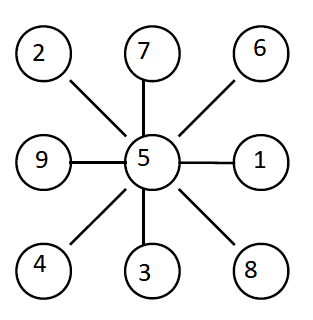
\includegraphics[scale=0.35]{2s.png}}
\end{figure}
\end{center}
8. По правилу магического квадрата в центре должно стоять число 6, далее подбираем.
\begin{center}
\begin{figure}[h!]
\center{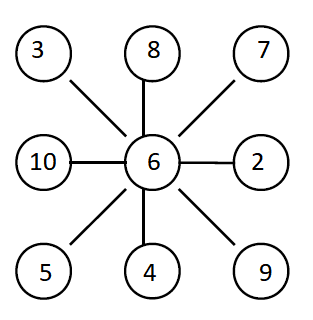
\includegraphics[scale=0.35]{22s.png}}
\end{figure}
\end{center}
9. Это числа $2\cdot2=4,\ 2\cdot3=6,\ 2\cdot2\cdot2=8,\ 3\cdot3=9,\ 2\cdot2\cdot3=12,\ 2\cdot2\cdot2\cdot2=16,\ 2\cdot3\cdot3=18.$\\
10. Это числа $2\cdot2\cdot2=8,\ 2\cdot5=10,\ 2\cdot2\cdot2\cdot2=16,\ 2\cdot2\cdot5=20, 5\cdot5=25.$\\
11. Будем раскладывать на более мелкие множители: $405=5\cdot81=5\cdot9\cdot9=5\cdot9\cdot3\cdot3.$ Получилось то, что надо: $5+9+3+3=20.$\\
12. Будем раскладывать на более мелкие множители: $575=5\cdot115=5\cdot5\cdot23.$ Сумма получилась $5+5+23=33$ меньше необходимой, так что добавим в качестве множителей недостающее число единиц: $575=5\cdot5\cdot23\cdot1\cdot1\cdot1\cdot1,$ тогда $5+5+23+1+1+1+1=37.$\\
13. Произведём 8 фиксированных переливаний, не зависящих от объёма второго кувшина. В конце этих действий если он окажется пустым, то он был 5-литровым, а в противном случае --- 6-литровым.
\begin{center}
\begin{figure}[h!]
\center{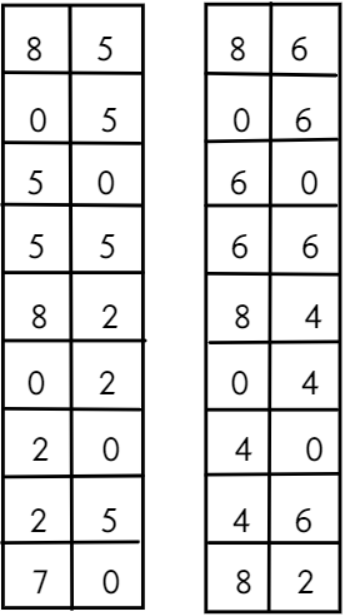
\includegraphics[scale=0.35]{s.png}}
\end{figure}
\end{center}

ewpage

oindent14. Произведём 8 фиксированных переливаний, не зависящих от объёма второго кувшина. В конце этих действий если он окажется пустым, то он был 3-литровым, а в противном случае --- 4-литровым.
\begin{center}
\begin{figure}[h!]
\center{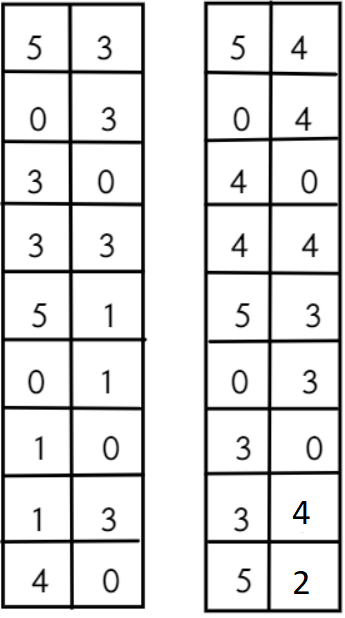
\includegraphics[scale=0.35]{ss.png}}
\end{figure}
\end{center}
15. Первый участник сыграет с остальными 13 партий, второй --- ещё 12 партий (партия с первым уже посчитана), третий 11 и так далее. Значит, необходимо найти сумму $13+12+11+\ldots+2+1.$ Её удобно найти, разбив числа на 6 пар с суммой 14 (и число 7 отдельно): $(13+1)+(12+2)+\ldots+(8+6)+7=14\cdot6+7=91.$\\
16. За один круг первая команда сыграет с остальными 15 матчей, вторая --- ещё 14 матчей (матч с первой уже посчитан), третья 13 и так далее. Значит, необходимо найти сумму $15+13+12+\ldots+2+1.$ Её удобно найти, разбив числа на 7 пар с суммой 16 (и число 8 отдельно): $(15+1)+(14+2)+\ldots+(9+7)+8=16\cdot7+8=120.$ Так как каждая команда сыграет с каждой по 2 матча, полученный ответ необходимо умножить на 2: $120\cdot2=240.$\\
17. Будем ставить маленькие числа рядом с большими и постепенно заполним картинку.
\begin{center}
\begin{figure}[h!]
\center{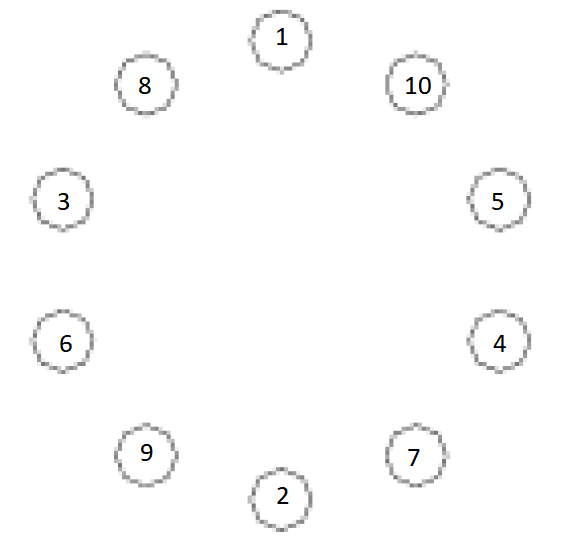
\includegraphics[scale=0.35]{3s.png}}
\end{figure}
\end{center}
18. Будем ставить маленькие числа рядом с большими и постепенно заполним картинку.
\begin{center}
\begin{figure}[h!]
\center{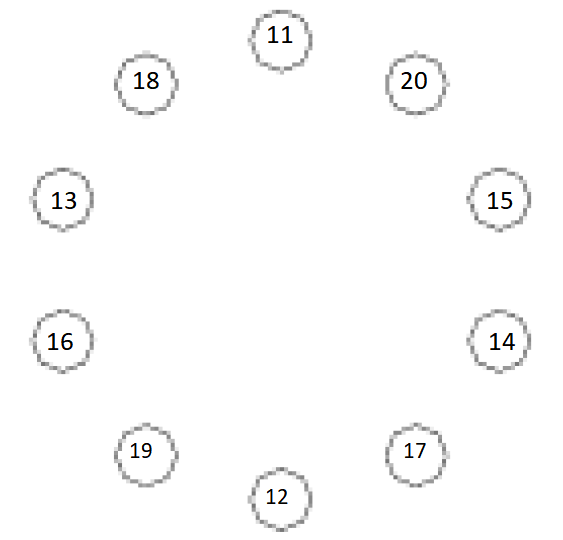
\includegraphics[scale=0.35]{33s.png}}
\end{figure}
\end{center}
19. На рисунке можно увидеть 12 квадратиков $1\times1,$ 6 квадратов $2\times2$ и 2 квадрата $3\times3,$ всего $12+6+2=20$ квадратов.\\
20. На рисунке можно увидеть 9 квадратиков $1\times1,$ 4 квадрата $2\times2$ и 1 квадрат $3\times3,$ всего $9+4+1=14$ квадратов.\\
21. На первое место есть 4 способа выбрать цифру, на второе и третье --- по 5 (0 нельзя ставить на первое место, но можно на второе и третье), значит всего таких чисел $4\cdot5\cdot5=100.$\\
22. На первое место есть 9 способов выбрать цифру (без 0), на второе 10, на третье --- 5 (только чётные цифры), значит всего таких чисел $9\cdot10\cdot5=450.$\\
23. Эта разность равна $9876-1023=8853.$\\
24. Эта сумма равна $9876-1023=10899.$\\
25. Раз брюнет говорил с Беловым, брюнетом может быть только Рыжов. Тогда Белов должен быть рыжим, а Чернов --- блондином.\\
26. Если первым бал заяц, то в высказывании второй белки оба утверждения ложны (заяц не мог быть ещё и вторым, а лось не мог тоже быть первым). Если первой была лиса, то в утверждении первой белки ложны оба утверждения (заяц не мог быть тоже первым, лиса не могла быть ещё и второй). Значит, первым был лось и верно второе утверждение первой белки, поэтому лиса была второй.\\
27. Подберём знаки так, чтобы получилось нужное произведение: $5\cdot4\cdot(3+2\cdot1) = 100.$\\
28. Подберём знаки так, чтобы из 48 сделать 58: $6\cdot8+20:4\cdot2 = 58.$\\
29. Количество прошедших дней должно делиться на 2, 4 и на 5. Первое подходящее число равно 20, оно даёт остаток 6 при делении на 7, значит они встретятся в $\text{вт}+6=\text{пн}$.\\
30. Количество прошедших дней должно делиться на 6, 3 и на 4. Первое подходящее число равно 12, оно даёт остаток 5 при делении на 7, значит они встретятся в $\text{сб}+5=\text{чт}$.\\
31. Поставим в первую строчку 11 и 6, далее заполняется однозначно.
\begin{center}
\begin{figure}[ht!]
\center{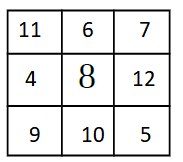
\includegraphics[scale=0.35]{5s.png}}
\end{figure}
\end{center}
32. Согласно правилу магического квадрата в центре должно стоять среднее число 4, а все суммы должны быть равны $4\cdot3=12.$ Поставим в первую строчку 7 и 2, далее заполняется однозначно.
\begin{center}
\begin{figure}[ht!]
\center{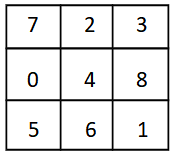
\includegraphics[scale=0.35]{55s.png}}
\end{figure}
\end{center}
33. Количество множителей равно $2012+1=2013$ (перед 9 стоят все числа от 1 до 2012, а также есть просто 9). Последняя цифра будет изменяться со следующей закономерностью: $9,\ 1,\ 9,\ 1,\ 9,\ldots$ При нечётном количестве множителей последняя цифра будет равна 9, значит сумма будет кончаться на $..9+1=..0$.\\
34. Количество множителей равно $2012+1=2013$ (перед 4 стоят все числа от 1 до 2012, а также есть просто 4). Последняя цифра будет изменяться со следующей закономерностью: $4,\ 6,\ 4,\ 6,\ 4,\ldots$ При нечётном количестве множителей последняя цифра будет равна 4, значит разность будет кончаться на $4-1=3.$\\
35. На первое место есть 9 способов выбрать цифру (без 0), на второе 10, на третье 1 (это точно 7), на четвёртое 10, на пятое --- 5 (эта цифра должна быть чётной), значит всего таких чисел $9\cdot10\cdot1\cdot10\cdot5=4500.$\\
36. На первое место можно поставить только 2 цифры 1 и 3, на второе 4 оставшихся, на третье --- 3, значит всего таких чисел $2\cdot4\cdot3=24.$\\
37. а) Наибольшей первой цифрой можно сделать 8, значит необходимо зачеркнуть 3,7,2 и получить число 8106.\\
б) Наименьшей первой цифрой можно сделать 2, а наименьшей второй --- 1, значит необходимо зачеркнуть 3,7,8 и получить число 2106.\\
38. а) Наибольшей первой цифрой можно сделать 9, а наибольшей второй --- 4, значит необходимо зачеркнуть 4,7,1 и получить число 9402.\\
б) Наименьшей первой цифрой можно сделать 1, значит необходимо зачеркнуть 4,7,9 и получить число 1402.\\
39. Пушкин точно стоит на первом месте и на количество способов никак не влияет. Выбрать 2 места из 4 для Маршака с Барто --- 3 способа (1 и 2, 2 и 3, 3 и 4). Выбрать порядок для Маршака и Барто --- 2 способа (Маршак-Барто и Барто-Маршак), как и для  Лермонтова с Некрасовым. Значит, всего расстановок $3\cdot2\cdot2=12.$\\
40. Пушкин точно стоит на первом месте и на количество способов никак не влияет. Выбрать 2 места из 4 для Бажова с Андерсеном --- 3 способа (1 и 2, 2 и 3, 3 и 4). Выбрать порядок для Бажова и Андерсена --- 2 способа (Бажов-Андерсен и Андерсен-Бажов), как и для  Гримма с Перро. Значит, всего расстановок $3\cdot2\cdot2=12.$\\
41. Каждой стороне, кроме двух соседних с выбранной вершиной, соответствует треугольник, значит их будет $20-2=18.$\\
42. Каждой стороне, кроме двух соседних с выбранной вершиной, соответствует треугольник, значит их будет $30-2=28.$\\
43. Согласно правилу магического квадрата все суммы должны быть равны $15\cdot3=45.$ Поставим в первый ряд числа 22 и 2, далее числа расставляются однозначно.
\begin{center}
\begin{figure}[ht!]
\center{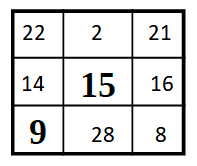
\includegraphics[scale=0.35]{7s.png}}
\end{figure}
\end{center}
44. Согласно правилу магического квадрата все суммы должны быть равны $13\cdot3=39,$ поэтому все числа расставляются однозначно.
\begin{center}
\begin{figure}[ht!]
\center{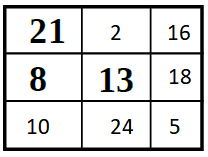
\includegraphics[scale=0.35]{77s.png}}
\end{figure}
\end{center}
45. Поставим первыми тремя числами первые 3 нечётных числа 1, 3 и 5, тогда последнее число равно $50-1-3-5=41.$\\
46. Поставим первыми тремя числами первые 3 нечётных числа 1, 3 и 5, тогда последнее число равно $56-1-3-5=47.$\\
47. Если бы можно брать одинаковые числа, мы бы взяли 5 раз по $120:5=24.$ Так как числа должны быть различными, будем их менять, сохраняя сумму: одно на 1 уменьшим, другое на 1 увеличим, одно на 2 уменьшим, другое на 2 увеличим. Получится набор $22,\ 23,\ 24,\ 25,\ 26.$\\
48. Если бы можно брать одинаковые числа, мы бы взяли 5 раз по $110:5=22.$ Так как числа должны быть различными, будем их менять, сохраняя сумму: одно на 1 уменьшим, другое на 1 увеличим, одно на 2 уменьшим, другое на 2 увеличим. Получится набор $20,\ 21,\ 22,\ 23,\ 24.$\\
49. Оставшиеся цифры в сумме дают $16-9-3-2=2,$ значит почти все они равны 0. Если это 2 и остальные 0, то 2 точно должно стоять на первом месте (там не может стоять 0), так что такое число только одно. Если это две 1, то одна из них точно стоит на первом месте, а для второй осталось $100-4=96$ свободных мест. Значит, всего таких чисел $96+1=97.$\\
50. Оставшиеся цифры в сумме дают $17-9-4-2=2,$ значит почти все они равны 0. Если это 2 и остальные 0, то 2 точно должно стоять на первом месте (там не может стоять 0), так что такое число только одно. Если это две 1, то одна из них точно стоит на первом месте, а для второй осталось $90-4=86$ свободных мест. Значит, всего таких чисел $86+1=87.$\\
51. Разобьём эту букву на горизонтальный (шляпку) и вертикальный (ножку) прямоугольники. Размеры горизонтального $70\times6,$ размеры вертикального --- $6\times54$ (для нахождения его высоты необходимо из высоты буквы Т вычесть толщину шляпки). Поэтому буква Т содержит $70\cdot6+6\cdot54=744$ клетки.\\
52. Разобьём эту букву на горизонтальный (шляпку) и вертикальный (ножку) прямоугольники. Размеры горизонтального $60\times8,$ размеры вертикального --- $8\times62$ (для нахождения его высоты необходимо из высоты буквы Т вычесть толщину шляпки). Поэтому буква Т содержит $60\cdot8+8\cdot62=976$ клеток.\\
53. Разобьём эту букву на горизонтальный (шляпку) и два вертикальных (ножки) прямоугольники. Размеры горизонтального $70\times6,$ размеры вертикальных --- $6\times54$ (для нахождения их высоты необходимо из высоты буквы П вычесть толщину шляпки). Поэтому буква П содержит $70\cdot6+6\cdot54\cdot2=1068$ клеток.\\
54. Разобьём эту букву на горизонтальный (шляпку) и два вертикальных (ножки) прямоугольники. Размеры горизонтального $60\times7,$ размеры вертикальных --- $7\times73$ (для нахождения их высоты необходимо из высоты буквы П вычесть толщину шляпки). Поэтому буква П содержит $60\cdot7+7\cdot73\cdot2=1442$ клетки.\\
55. Если бы можно брать одинаковые числа, мы бы взяли 5 раз по $375:5=75.$ Так как числа должны быть различными, будем их менять, сохраняя сумму: одно на 2 уменьшим, другое на 2 увеличим, одно на 4 уменьшим, другое на 4 увеличим. Получится набор $71,\ 73,\ 75,\ 77,\ 79.$\\
56. Если бы можно брать одинаковые числа, мы бы взяли 5 раз по $115:5=23.$ Так как числа должны быть различными, будем их менять, сохраняя сумму: одно на 2 уменьшим, другое на 2 увеличим, одно на 4 уменьшим, другое на 4 увеличим. Получится набор $19,\ 21,\ 23,\ 25,\ 27.$\\
57. Получить числа 7 и 36 можно только как $7:1=7$ и $4\times9=36.$ Тогда из остальных цифр нужно выбрать два, дающих в сумме третье так, чтобы оставшиеся два числа отличались на 4. Это можно сделать единственным способом.
\begin{center}
\begin{figure}[ht!]
\center{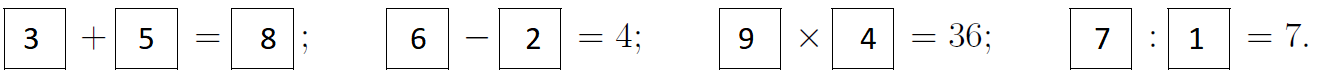
\includegraphics[scale=0.35]{11s.png}}
\end{figure}
\end{center}
58. Получить числа 5 и 16 можно только как $5:1=7$ и $8\times2=16.$ Тогда из остальных цифр нужно выбрать два, дающих в сумме 11 это могут быть только 7 и 4. Три оставшихся цифры как раз образуют пример на вычитание.
\begin{center}
\begin{figure}[ht!]
\center{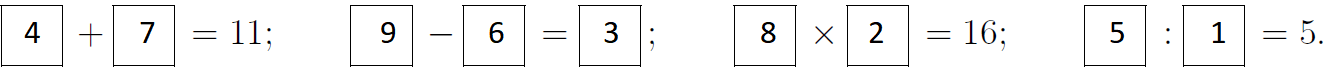
\includegraphics[scale=0.35]{111s.png}}
\end{figure}
\end{center}
59. Будем думать о том, сколько есть способов оставить цифры 4, 7 и 8, чтобы получилось число 478. Если оставить первую цифру 4 и первую цифру 7, с ними можно оставить 5 цифр 8. Если оставить первую цифру 4 и вторую цифру 7, с ними можно оставить 4 цифры 8. Если оставить вторую цифру 4, с ней можно оставить только вторую цифру 7 и с ними можно оставить 4 цифры 8. Таким образом, общее количество способов оставить число 478 равно $5+4+4=13.$\\
60. Будем думать о том, сколько есть способов оставить цифры 5, 6 и 9, чтобы получилось число 569. Если оставить первую цифру 5 и первую цифру 6, с ними можно оставить 5 цифр 9. Если оставить первую цифру 5 и вторую цифру 6, с ними можно оставить 4 цифры 9. Если оставить вторую цифру 5, с ней можно оставить только вторую цифру 6 и с ними можно оставить 4 цифры 9. Таким образом, общее количество способов оставить число 569 равно $5+4+4=13.$\\
61. В одном горизонтальном ряду 50 перегородок, а таких рядов $12-1=11,$ так как они разделяют 12 строк. Аналогично в одном вертикальном ряду 12 перегородок, а количество таких рядов равно $50-1=49,$ они разделяют 50 столбцов. Таким образом, общее количество перегородок равно $11\cdot50+49\cdot50=1138.$\\
62. В одном горизонтальном ряду 15 перегородок, а таких рядов $40-1=39,$ так как они разделяют 40 строк. Аналогично в одном вертикальном ряду 40 перегородок, а количество таких рядов равно $15-1=14,$ они разделяют 15 столбцов. Таким образом, общее количество перегородок равно $39\cdot15+14\cdot40=1145.$\\
63. Поделим с остатком: $2017:6=336$ (ост. 1). Значит, первые 2 цифры в этих числах точно равны 3 и 3. Осталось подобрать последние цифры так, чтобы сумма получилась 2017, например это можно сделать так: 333, 334, 336, 337, 338, 339.\\
64. Поделим с остатком: $2057:6=342$ (ост. 5). Значит, первые 2 цифры в этих числах точно равны 3 и 4. Осталось подобрать последние цифры так, чтобы сумма получилась 2057, например это можно сделать так: 340, 341, 342, 343, 344, 347.\\
65. Мужа Натальи зовут Михаил, его брата, а значит и деверя Натальи, зовут Георгий. Отца Георгия зовут Александр, его жену зовут Мария, её сестру, а значит свояченицу Александра, зовут Александра. Сына Александры зовут Виктор.\\
66. Мужа Анны зовут Максим, его брата, а значит и деверя Анны, зовут Александр. Отца Александра зовут Иван, его жену зовут Мария, её сестру, а значит свояченицу Ивана, зовут Александра. Сына Александры зовут Василий.\\
67. Можно взять прямоугольник $2\times5$ и переставить 2 клетки.
\begin{center}
\begin{figure}[ht!]
\center{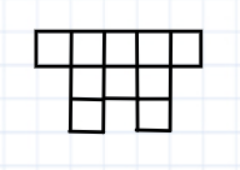
\includegraphics[scale=0.35]{1111.png}}
\end{figure}
\end{center}
68. Можно взять квадрат $3\times3$ и переставить 1 клетку.
\begin{center}
\begin{figure}[ht!]
\center{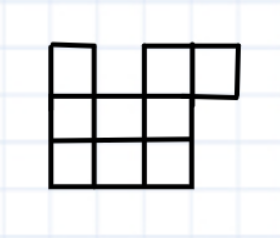
\includegraphics[scale=0.35]{11111.png}}
\end{figure}
\end{center}
69. Дно ванны имеет размер $3\text{дм}\times5\text{дм},$ а высота наименьшего бортика (через который нельзя переливать) --- 2дм, значит в ванну войдёт максимум $3\cdot5\cdot2=30\text{дм}^3=30$л.\\
70. Дно ванны имеет размер $3\text{дм}\times6\text{дм},$ а высота наименьшего бортика (через который нельзя переливать) --- 2дм, значит в ванну войдёт максимум $3\cdot6\cdot2=36\text{дм}^3=36$л.\\
71. Если бы дырки не было, то в прямоугольнике $30\times40$ было бы $30\cdot39+40\cdot29=2330$ перегородок (см. задачи 61-62). Дырка имеет размеры $(30-2\cdot4)\times(40-2\cdot4)=22\times32.$ Внутри неё <<пропадут>> $22\cdot31+32\cdot21=1354$ перегородки. Также не будет считаться перегородками периметр дырки: $(22+32)\cdot2=108.$ Итого в букве О останется $2330-1354-108=868$ перегородок.\\
72. Если бы дырки не было, то в прямоугольнике $20\times30$ было бы $20\cdot29+30\cdot19=1150$ перегородок (см. задачи 61-62). Дырка имеет размеры $(20-2\cdot4)\times(30-2\cdot4)=12\times22.$ Внутри неё <<пропадут>> $12\cdot21+22\cdot11=494$ перегородки. Также не будет считаться перегородками периметр дырки: $(12+22)\cdot2=68.$ Итого в букве О останется $1150-494-68=588$ перегородок.\\
73. В первом случае в пересечении образуется квадрат, раз его площадь равна $4\text{м}^2,$ его сторона равна 2м. Во втором случае образуется прямоугольник, горизонтальная сторона которого также равна 2м, а значит вертикальная сторона равна $14:2=7$м, она же является стороной меньшего ковра. Значит, сторона большего ковра равна $7\cdot2=14$м и сторона комнаты равна $12+2+5=19$м.
\begin{center}
\begin{figure}[ht!]
\center{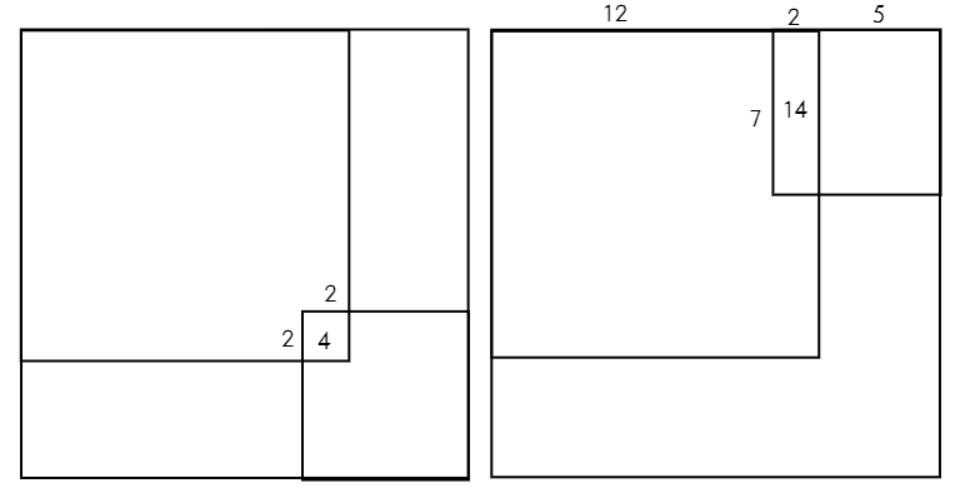
\includegraphics[scale=0.35]{sq.png}}
\end{figure}
\end{center}

ewpage

oindent74. В первом случае в пересечении образуется квадрат, раз его площадь равна $9\text{м}^2,$ его сторона равна 3м. Во втором случае образуется прямоугольник, горизонтальная сторона которого также равна 3м, а значит вертикальная сторона равна $15:3=5$м, она же является стороной меньшего ковра. Значит, сторона большего ковра равна $5\cdot2=10$м и сторона комнаты равна $7+3+2=12$м.
\begin{center}
\begin{figure}[ht!]
\center{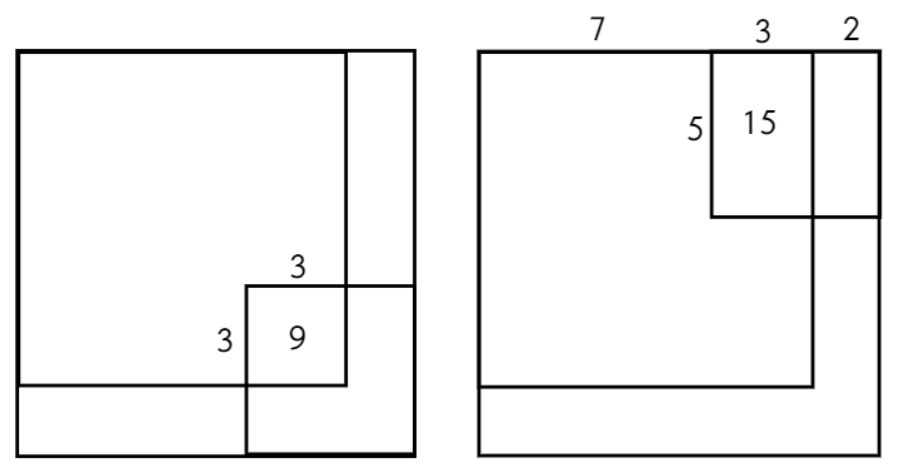
\includegraphics[scale=0.35]{sq1.png}}
\end{figure}
\end{center}
75. Если одно из чисел получается из другого добавлением 0, оно в 10 раз больше. Пусть меньшее число равно $x,$ тогда $x+10x=8481,\ 11x=8481,\ x=171.$ Значит, эти числа равны 171 и 1710.\\
76. Приложить друг к другу два прямоугольника можно тремя способами. В первых двух случаях прямоугольники одинаковые, а в третьем --- это прямоугольники $4\times1$ и $16\times4$(он тоже имеет пузатость $4:1$). Получим пузатости $8:1,\ 2:1,\ 17:4.$
\begin{center}
\begin{figure}[ht!]
\center{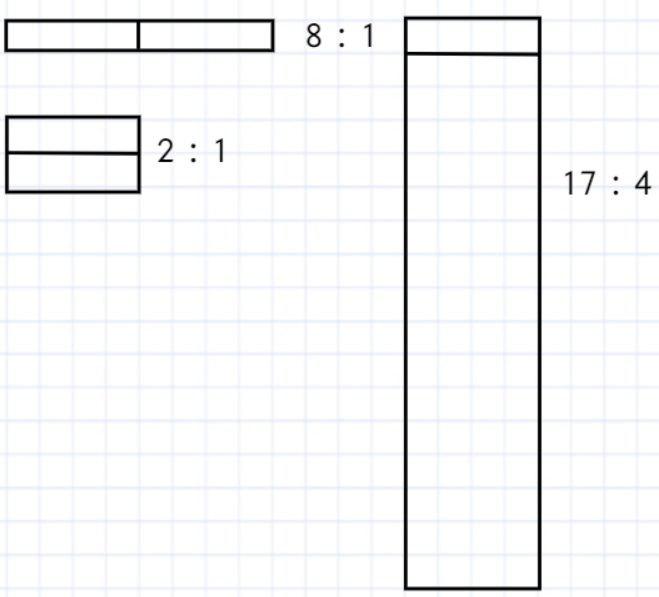
\includegraphics[scale=0.35]{puz1.png}}
\end{figure}
\end{center}
77. Приложить друг к другу два прямоугольника можно тремя способами. В первых двух случаях прямоугольники одинаковые, а в третьем --- это прямоугольники $3\times1$ и $9\times3$(он тоже имеет пузатость $3:1$). Получим пузатости $6:1,\ 3:2,\ 10:3.$
\begin{center}
\begin{figure}[ht!]
\center{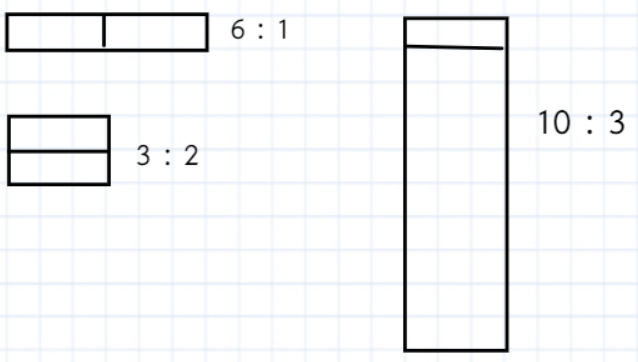
\includegraphics[scale=0.35]{puz.png}}
\end{figure}
\end{center}
78. В первом случае трёхзначным будет само первое число $N.$ Все такие числа подходят, так как $N+937$ в этом случае уже будут четырёхзначными. Всего трёхзначных чисел 900. Во втором случае трёхзначным будет только второе число $N+937.$ В этом случае подходят только числа $N$ от 1 до 62 (если $N=63,$ то $N+937=1000$ уже четырёхзначное и трёхзначных чисел вообще нет). Значит, всего существует $900+62=962$ таких числа.\\
79. В первом случае трёхзначным будет само первое число $N.$ Все такие числа подходят, так как $N+973$ в этом случае уже будут четырёхзначными. Всего трёхзначных чисел 900. Во втором случае трёхзначным будет только второе число $N+973.$ В этом случае подходят только числа $N$ от 1 до 26 (если $N=27,$ то $N+973=1000$ уже четырёхзначное и трёхзначных чисел вообще нет). Значит, всего существует $900+26=926$ таких чисел.\\
80. Произведение 20 можно получить двумя способами: $5\cdot4\cdot1\cdot1\cdot1$ и $5\cdot2\cdot2\cdot1\cdot1.$ В первом случае 4 точно надо поставить на последнее место (так как число чётное), а затем выбрать одно из 4 доступных мет для цифры 5 (остальные места займут 1). Таких чисел будет 4. Во втором случае надо сначала поставить одну из цифр 2 на последнее место, затем выбрать место для второй 2 (4 способа), а потом для цифры 5 (3 способа). Таких чисел будет $4\cdot3=12.$ Значит, всего таких чисел существует $4+12=16.$\\
81. Произведение 28 можно получить двумя способами: $7\cdot4\cdot1\cdot1\cdot1$ и $7\cdot2\cdot2\cdot1\cdot1.$ В первом случае 4 точно надо поставить на последнее место (так как число чётное), а затем выбрать одно из 4 доступных мет для цифры 7 (остальные места займут 1). Таких чисел будет 4. Во втором случае надо сначала поставить одну из цифр 2 на последнее место, затем выбрать место для второй 2 (4 способа), а потом для цифры 7 (3 способа). Таких чисел будет $4\cdot3=12.$ Значит, всего таких чисел существует $4+12=16.$\\
82. Впервые все цифры на табло часов окажутся разными в 13:02:45, через 2 минуты и 38 секунд.\\
83. Впервые все цифры на табло часов окажутся разными в 12:03:45, через 3 минуты и 37 секунд.\\
84. Разница между количеством мест в первом и втором поездах равна $295-236=59.$ В двух вагонах должно быть больше $30\cdot2=60$ мест, значит это количество мест в одном вагоне. Поэтому всего вагонов $(236+295+472):59=17.$\\
85. Разница между количеством мест в первом и втором поездах равна $318-265=53.$ В двух вагонах должно быть больше $30\cdot2=60$ мест, значит это количество мест в одном вагоне. Поэтому всего вагонов $(265+318+477):53=20.$\\
86. Сначала посчитаем, сколько клеток в исходном прямоугольнике: их 37. После это надо приложить букву $L$ всеми возможными способами и посмотреть, сколько клеток она может добавить. При этом надо не забывать, что фигуру можно как поворачивать, так и переворачивать.
\begin{figure}[ht!]
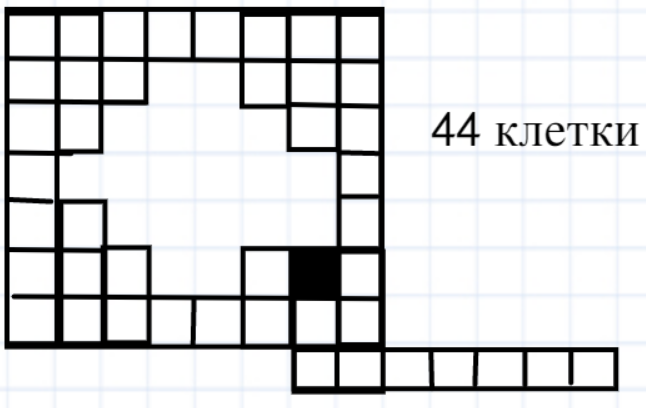
\includegraphics[scale=0.35]{l1.png} 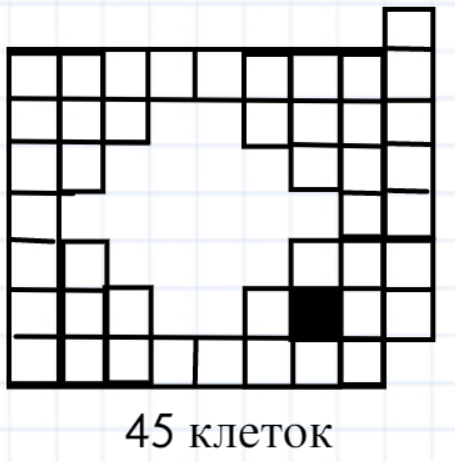
\includegraphics[scale=0.35]{l2.png}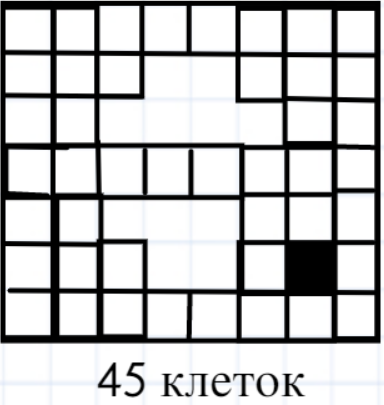
\includegraphics[scale=0.35]{l3.png}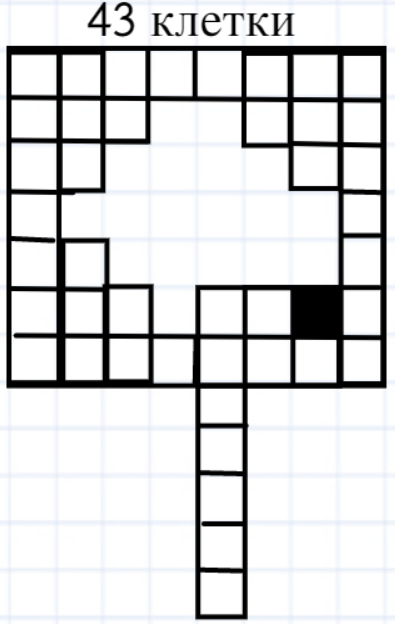
\includegraphics[scale=0.35]{l4.png}\end{figure}
\begin{figure}[ht!]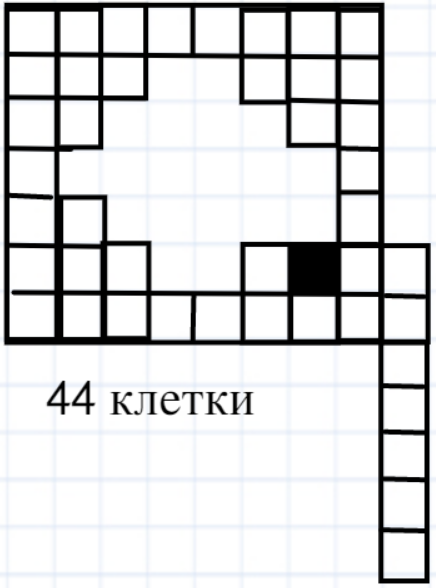
\includegraphics[scale=0.35]{l5.png} 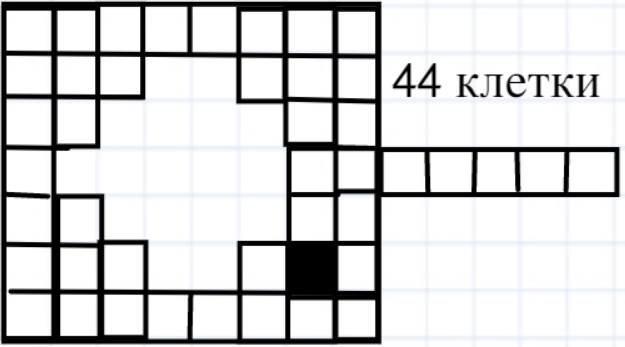
\includegraphics[scale=0.35]{l6.png}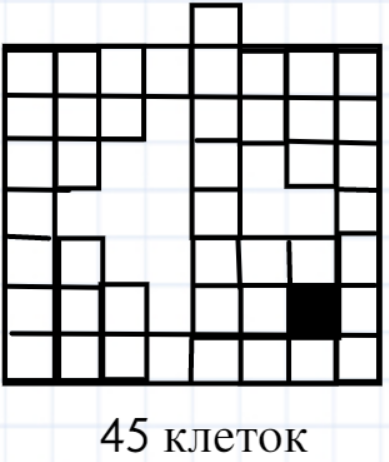
\includegraphics[scale=0.35]{l7.png}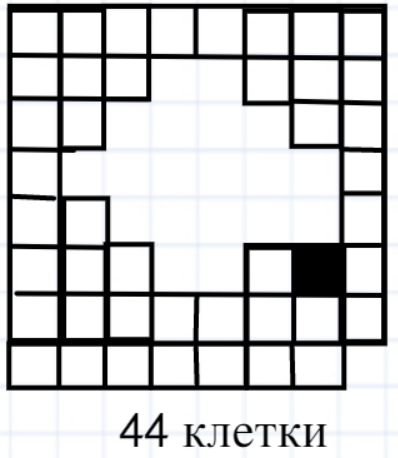
\includegraphics[scale=0.35]{l8.png}
\end{figure}\\
Как мы видим, возможны всего три варианта: 43, 44 или 45 клеток.

ewpage
oindent
87. Сначала посчитаем, сколько клеток в исходном прямоугольнике: их 39. После это надо приложить букву $P$ всеми возможными способами и посмотреть, сколько клеток она может добавить. При этом надо не забывать, что фигуру можно как поворачивать, так и переворачивать.
\begin{figure}[ht!]
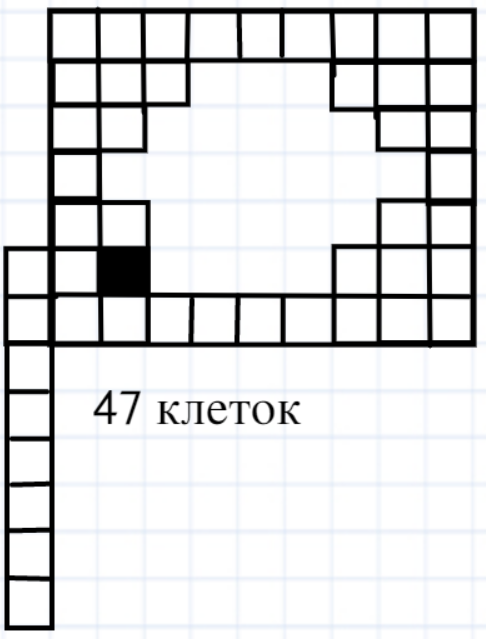
\includegraphics[scale=0.35]{ll1.png} 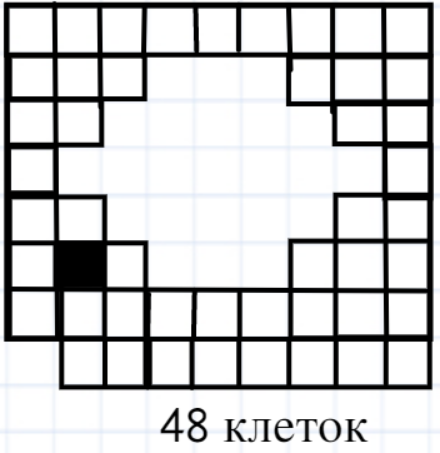
\includegraphics[scale=0.35]{ll2.png}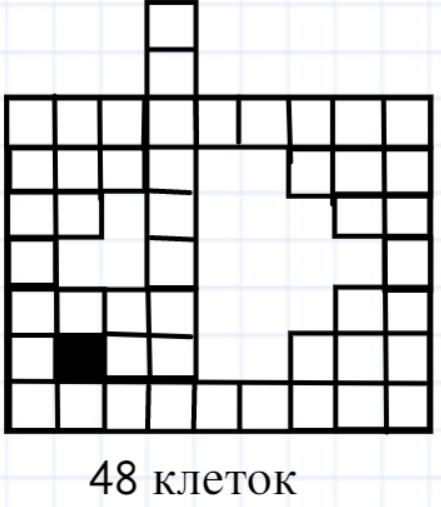
\includegraphics[scale=0.35]{ll3.png}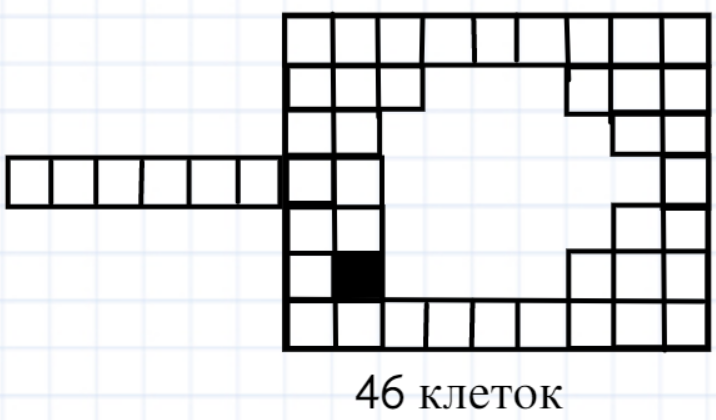
\includegraphics[scale=0.35]{ll4.png}\end{figure}
\begin{figure}[ht!]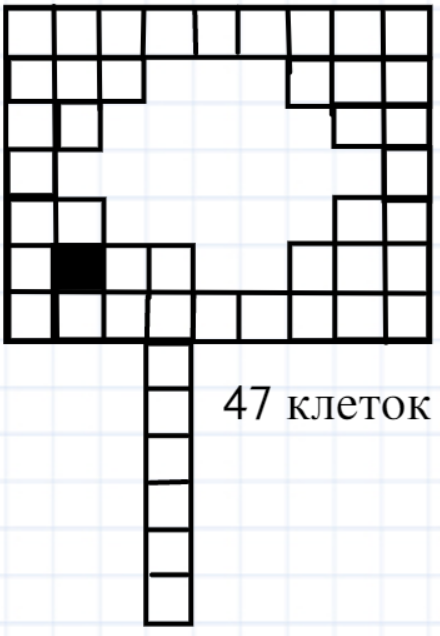
\includegraphics[scale=0.35]{ll5.png} 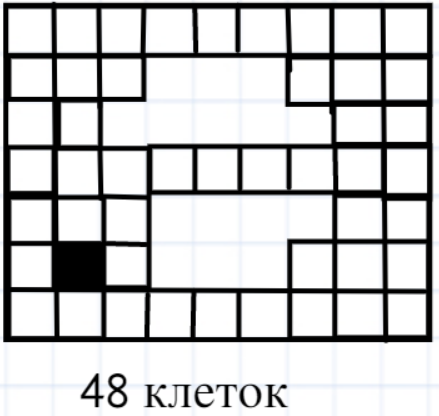
\includegraphics[scale=0.35]{ll6.png}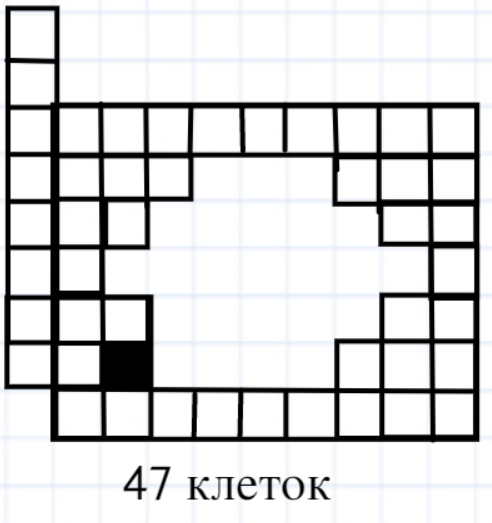
\includegraphics[scale=0.35]{ll7.png}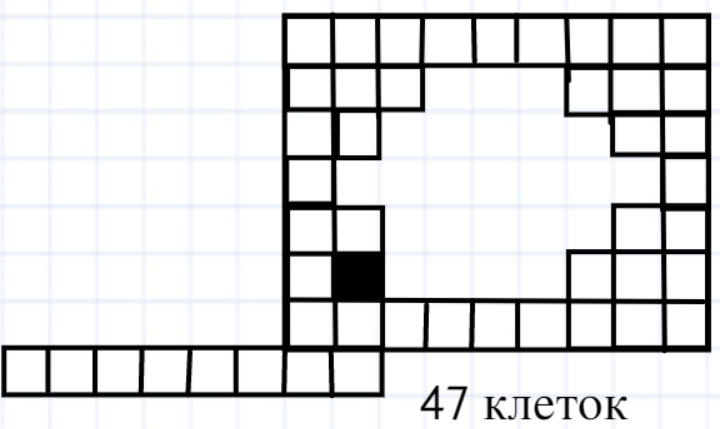
\includegraphics[scale=0.35]{ll8.png}
\end{figure}\\
Как мы видим, возможны всего три варианта: 46, 47 или 48 клеток.\\
88. У любого года XXI века вторая цифра равна 0, а значит и все произведения всегда равны 0.\\
89. У любого года XXI века вторая цифра равна 0, а значит и все произведения всегда равны 0.\\
90. При приведённых условиях возможны всего 2 ситуации, изображённые ниже.
\begin{center}
\begin{figure}[ht!]
\center{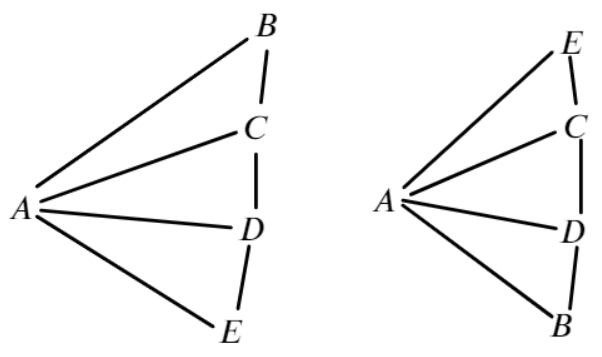
\includegraphics[scale=0.35]{dor1.png}}
\end{figure}
\end{center}
Как видно из картинки, выполняется утверждение Б. Отметим, что утверждение Г было бы верно, если бы из $C$ можно было бы попасть {\bf только в один} из городов $A$ и $D.$\\
91. При приведённых условиях возможны всего 2 ситуации, изображённые ниже.
\begin{center}
\begin{figure}[ht!]
\center{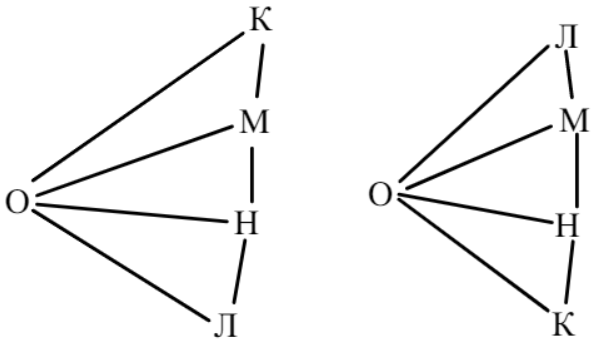
\includegraphics[scale=0.35]{dor2.png}}
\end{figure}
\end{center}
Как видно из картинки, выполняется утверждение Б. Отметим, что утверждение Г было бы верно, если бы из М можно было бы попасть {\bf только в один} из городов Н и О.\\
92. В записке написана ложь, значит барон М. сказал правду, когда сказал, что неправда, что А и Б одновременно сидели на трубе. Значит, А и Б одновременно на трубе не сидели, правильный ответ В.\\
93. В записке написана ложь, значит кучер сказал правду, когда сказал, что неправда, что А и Б одновременно НЕ сидели на трубе. Значит, А и Б одновременно на трубе сидели, правильный ответ А.\\
94. Нитки и лампочки могут лежать только в коробке с этикеткой Г, значит нитки и иголки лежат в коробке с этикеткой Л.\\
95. Книжки и шапочки могут лежать только в коробке с этикеткой Т.\\
96. Числа 400 и 401 на 3 не делятся, значит это число 402.\\
97. Необходимо вытащить 9 шаров (если каждого цвета максимум по 4 шара, то шаров максимум 8). Если вытащить 8 шаров, то среди них могут быть только по 4 шара каждого цвета.\\
98. Самой маленькой первой цифрой можно сделать 3, самой маленькой второй --- 0, поэтому надо вычеркнуть цифры 5, 8, 7 и 6.\\
99. Подбором найдём, что если 568 поделить на 238, получится 2 и остаток 92.\\
100. Необходимо ставить большие цифры как можно дальше, получится число 200034.\\
101. На нижней белой грани должна стоять цифра 2, так как она окажется напротив 5. Значит, на чёрных гранях могут стоять только цифры 3, 4, 5 и 6 (при этом цифры, дающие в сумме 7, не могут стоять на них обе). Наибольшая разность получится, если поставить на них цифры 3 и 6, она равна $6-3=3.$\\
102. Кубик собрать сможет тот из мальчиков, чьё количество кубиков можно получить перемножив 3 одинаковых числа. Поэтому кубик сможет собрать Вася, так как $3\cdot3\cdot3=27.$\\
103. У сыновей дедушки должно быть одинаковое отчество. Повторяется только отчество <<Игоревич>>, поэтому дедушку зовут Игорь.\\
104. На правой чёрной грани должна стоять цифра 4, так как она окажется напротив 3. На нижней белой грани должна стоять цифра 5, так как она окажется напротив 2. Значит, на второй чёрной грани могут стоять только цифры 1 и 6. Наибольшая разность получится, если поставить на неё цифру 1, она равна $4-1=3.$\\
105. Затянутся в узел те верёвки, которые над собой находятся сначала сверху, а потом снизу. Это верёвки на картинках Б и В.\\
106. Затянутся в узел те верёвки, которые над собой находятся сначала сверху, а потом снизу. Это верёвки на картинках А и В.\\
107. Победить ни Алёшу, ни Добрыню Соловей-разбойник не мог, при этом Илья Муромец его победить мог, так что правильные ответы --- А и Г.\\
108. Победить ни Василису Прекрасную, ни Василису Премудрую Баба Яга не могла, при этом победить Кикимору она могла, так что правильные ответы --- В и Г.\\
109. Общая стоимость марок равна $18+21+24+27+30+33=153$ рубля. Значит, необходимо убрать марку нечётной стоимости так, чтобы оставшиеся можно было разбить на две равные по стоимости группы. Это можно сделать только убрав марку стоимостью 27 рублей и разбив остальные следующим образом: $30+33=18+21+24.$\\
110. Общая стоимость марок равна $20+24+28+32+36+40=180$ рублей. Значит, необходимо убрать марку чётной стоимости так, чтобы оставшиеся можно было разбить на две равные по стоимости группы. Это можно сделать двумя способами: убрав марку стоимостью 36 рублей и разбив остальные на группы $40+32=20+24+28$ или убрав марку стоимость 28 рублей и разбив остальные на группы $40+36=20+24+32.$\\
111. Чтобы увидеть дырки на первой и на третьей картинке, необходимо убрать $3\cdot4=12$ кубиков, но при этом 2 кубика, находящиеся в нижнем слое в левом и правом рядах посередине будут посчитаны по 2 раза. Значит, необходимо убрать $12-2=10$ кубиков и их останется $3\cdot3\cdot3-10=17.$\\
112. Чтобы увидеть дырки на первой и на третьей картинке, необходимо убрать $3\cdot4=12$ кубиков, но при этом 2 кубика, находящиеся в левом слое в верхнем и нижнем рядах посередине будут посчитаны по 2 раза. Значит, необходимо убрать $12-2=10$ кубиков и их останется $3\cdot3\cdot3-10=17.$\\
113. Число сотен может не измениться при умножении на число тысяч только если число тысяч равно 1 или число сотен равно 0. Число десятков вдвое меньше, чем число тысяч, поэтому число тысяч не может быть равно 1. Значит, число сотен равно 0. Число единиц на 7 больше числа тысяч, при этом число тысяч должно быть чётным, значит оно равно 2 (иначе число единиц будет больше 10, что невозможно). Таким образом, число тысяч равно 2, число сотен равно 0, число десятков равно $2:2=1,$ число единиц равно $2+7=9,$ так что это число 2019.\\
114. Число десятков может не измениться при умножении на число тысяч только если число тысяч равно 1 или число десятков равно 0. Число сотен втрое меньше, чем число тысяч, поэтому число тысяч не может быть равно 1. Значит, число десятков равно 0. Число единиц на 5 больше числа тысяч, при этом число тысяч должно быть кратно трём, значит оно равно 3 (иначе число единиц будет больше 10, что невозможно). Таким образом, число тысяч равно 3, число сотен равно $3:3=1,$ число десятков равно 0, число единиц равно $3+5=8,$ так что это число 3108.\\
115. В каждом большом квадрате должны быть представлены все фигуры и все количества от 1 до 4, таким образом необходимо заполнить пустые квадратики следующим образом: 1 ромб, 4 креста, 3 треугольника, 2 ромба.\\
116. Раз он не выполнил обещание, он не сделал ничего из обещанного, правильный ответ б).\\
117. Судя по развёртке, напротив грани с цифрой 1 будет находиться грань с цифрой 6.\\
118. Изобразим описанный маршрут.
\begin{center}
\begin{figure}[ht!]
\center{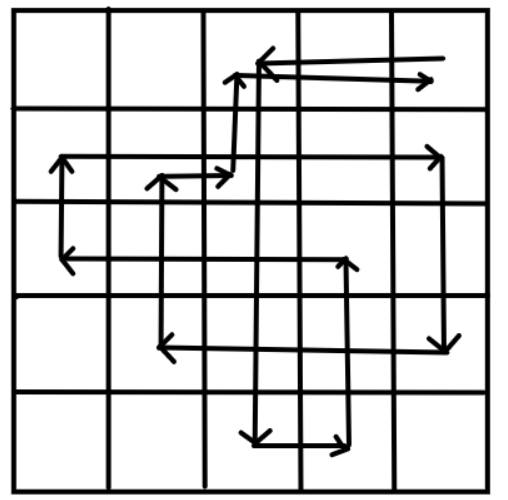
\includegraphics[scale=0.35]{put.png}}
\end{figure}
\end{center}
Как видно из картинки, муравьишка не побывал на 6 клетках.\\
119.Если нарисовать все цифры так, как они выглядят на табло, получим следующие соотношения: цифра 1 --- 2 лампочки, цифра 2 --- 5 лампочек, цифра 3 --- 5 лампочек, цифра 4 --- 4 лампочки, цифра 5 --- 5 лампочек, цифра 6 --- 6 лампочек, цифра 7 --- 3 лампочки, цифра 8 --- 7 лампочек, цифра 9 --- 6 лампочек, цифра 0 --- 6 лампочек. Поэтому нам подойдут такие 20 чисел: 14, 41, 27, 72, 28, 82, 37, 73, 38, 83, 46, 64, 49, 94, 40, 04, 57, 75, 58, 85.\\
120. В каждом из слоёв изначально было по $4\cdot4=16$ кубиков, а осталось (сверху вниз) $1\cdot1=1,\ 2\cdot2=4,\ 3\cdot3=9,\ 4\cdot4=16.$ Значит, убрали $(16-1)+(16-4)+(16-9)+(16-16)=34$ кубика.\\
121. В $1\text{см}^2$ содержится $2\cdot2=4$ клетки, значит необходимо нарисовать десятиугольник, состоящий из $4\cdot10+4:2=42$ клеток. Один из возможных примеров изображён ниже.
\begin{center}
\begin{figure}[ht!]
\center{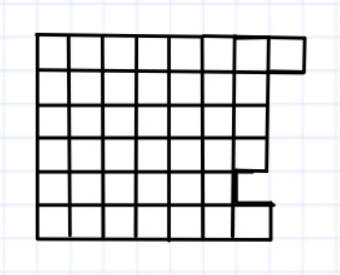
\includegraphics[scale=0.35]{2222.png}}
\end{figure}
\end{center}
122. У Порфирия получился клетчатый прямоугольник с размерами $200:10=20$ на $100:10=10.$ В центрах клеток будет $20\cdot10=200$ саженцев. Узлов сетки будет $(10-1)\cdot(20-1)=171,$ значит всего саженцев будет $200+171=371.$\\
123. Все оставшиеся кепки синие, значит красных кепок точно нет и утверждение 1) верно. Из красных вещей остались только футболки, но это не значит, что других футболок не осталось, поэтому утверждение 2) может быть как верно, так и неверно. Зелёных кроссовок в магазине в принципе не было, так что про утверждение 3) ничего нельзя сказать. Красными могут быть только футболки, так что все оставшиеся шорты могут быть только синими, утверждение 4) верно. Некоторые футболки могут быть синими, но могут и не быть. Таким образом, точно верны только утверждения 1) и 4).\\
124. Перечислим их все: 3000, 2100, 2010, 2001, 1200, 1020, 1002, 1110, 1101, 1011. Таким образом, их 10.\\
125. Перечислим их все: 9997, 9979, 9799, 7999, 9988, 9898, 9889, 8998, 8989, 8899. Таким образом, их 10.\\
126. Перечислим их все: $ABC,\ ABN,\ AMC,\ AMN,\ MBN,\ MBC,\ MNC,\ CNA.$ Таким образом, их 8.
\begin{center}
\begin{figure}[ht!]
\center{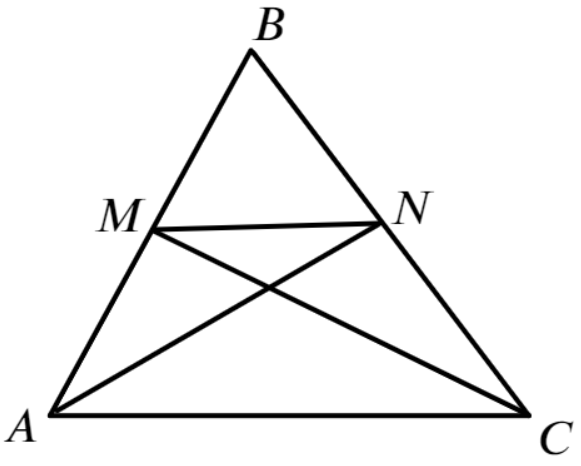
\includegraphics[scale=0.35]{tr.png}}
\end{figure}
\end{center}
127.  Пусть длина отрезка $AB$ равна $x,$ тогда $BC=2x,\ CD=4\cdot2x=8x$ и $x+2x+8x=33,\ 11x=33,\ x=3$ см. Таким образом, отрезки $AB,\ BC$ и $CD$ равны 3см, $2\cdot3=6$см и $8\cdot3=24$см.\\
128. Пусть длина отрезка $BC$ равна $x,$ тогда $AB=2x,\ AC=2x-x=x,\ CD=4x,\ BD=4x-x=3x$ и $x+x+3x=25,\ 5x=25,\ x=5$ см. Таким образом, отрезки $AC,\ CB$ и $BD$ равны 5см, 5см и $3\cdot5=15$см.\\
129. Если Марк сказал правду, то Лев тоже сказал правду, чего быть не может. Значит, Марк солгал, а Лев сказал правду и им больше 9, но не больше 10 лет. Поэтому им исполнилось ровно 10 лет.\\
130. Если Рон сказал правду, то Тук тоже сказал правду, чего быть не может. Значит, Рон солгал, а Тук сказал правду и им больше 11, но не больше 12 лет. Поэтому им исполнилось ровно 12 лет.\\
131. Если Аня взяла конфету, то она должна была сказать правду, но она сказала, что конфету взял Борис. Если конфету взял Борис, то Аня сказала правду, значит конфету должна была взять она сама. Таким образом, конфету могла взять только Вика.\\
132. Общая сторона у верхнего и бокового слоя должна быть равна 11 (общий делитель 77 и 55). Значит, изначально коробка имела размеры $7\times11\times6.$ После того, как съели верхний слой, размеры стали $7\times11\times5,$ а после съедения бокового --- $6\times11\times5.$ Таким образом, в переднем слое дети съедят $6\cdot5=30$ кусочков сахара.\\
133. Общая сторона у верхнего и бокового слоя должна быть равна 11 (общий делитель 55 и 33). Значит, изначально коробка имела размеры $5\times11\times4.$ Таким образом, осталось $5\cdot11\cdot4-55-33=132$ кусочка.\\
134. Разложим число 210 на множители: $210=2\cdot5\cdot3\cdot7.$ Значит это число равно 5372.\\
135. Нарисуем картинку, следуя указаниям.
\begin{center}
\begin{figure}[ht!]
\center{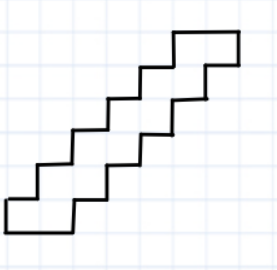
\includegraphics[scale=0.35]{321.png}}
\end{figure}
\end{center}
Площадь полученной фигуры равна $12\text{ м}^2.$

ewpage
oindent
136. Нарисуем картинку, следуя указаниям.
\begin{center}
\begin{figure}[ht!]
\center{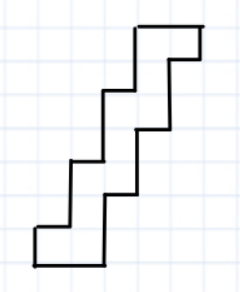
\includegraphics[scale=0.35]{123.png}}
\end{figure}
\end{center}
Площадь полученной фигуры равна $11\text{ м}^2.$\\
137. Общее количество клеток в трёх фигурках нечётно, поэтому сложим их так, чтобы ось симметрии делила клетки пополам.
\begin{center}
\begin{figure}[ht!]
\center{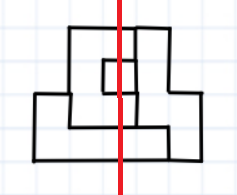
\includegraphics[scale=0.35]{666s.png}}
\end{figure}
\end{center}
138. Изначально число очевидно делится на 533, далее необходимо знать разложение $1001=7\cdot11\cdot13.$ Делимость на 101 находить необязательно. В конце всегда можно дописать множитель 1. Таким образом, получим $533533533533=7\cdot11\cdot13\cdot533\cdot101\cdot9901\cdot1.$\\
139. Изначально число очевидно делится на 517, далее необходимо знать разложение $1001=7\cdot11\cdot13.$ Делимость на 101 находить необязательно. В конце всегда можно дописать множитель 1. Таким образом, получим $517517517517=7\cdot11\cdot13\cdot517\cdot101\cdot9901\cdot1.$\\
140. Васильев прибежал позже Борисова, а значит не мог выиграть забег. Если Петров прибежал раньше Васильева, то не мог быт последним. Таким образом, заведомо ложны утверждения а) и г).\\
141. Если Алексей съел больше Бориса, то больше всех съел Дмитрий, потом Алексей, потом Борис, а потом Сергей. Остальные утверждения могут быть как верны, так и ложны. Таким образом, заведомо истинно только утверждение г).\\
142. В клеточках сторона квадрата равна $20\cdot2=40$ клеточек. Внутренняя часть имеет сторону $40-2\cdot2=36$ клеточек, поэтому в каёмке $40\cdot40-36\cdot36=304$ клеточки.\\
143. В клеточках сторона квадрата равна $17\cdot2=34$ клеточки. Внутренняя часть имеет сторону $34-2\cdot3=28$ клеточек, поэтому в каёмке $34\cdot34-28\cdot28=372$ клеточки.\\
144. Один из возможных вариантов --- <<буква Ш>>.
\begin{center}
\begin{figure}[ht!]
\center{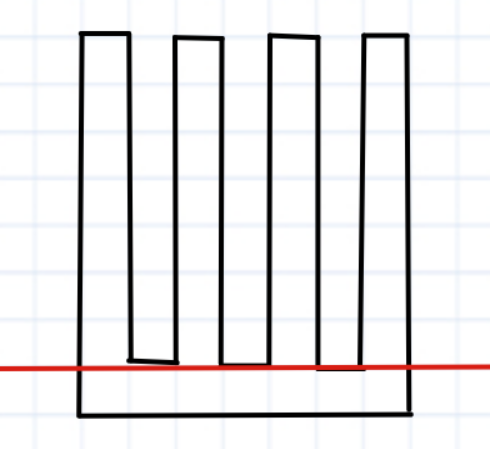
\includegraphics[scale=0.35]{qq.png}}
\end{figure}
\end{center}
ewpage
oindent
145. Один из возможных вариантов --- <<буква Ш>>.
\begin{center}
\begin{figure}[ht!]
\center{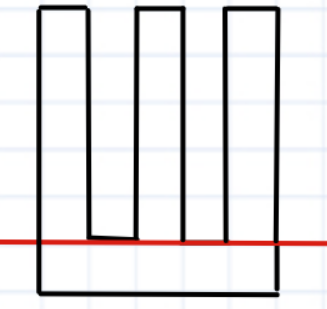
\includegraphics[scale=0.35]{qqq.png}}
\end{figure}
\end{center}
146. Самой маленькой первой цифрой можно сделать 2, самой маленькой второй 8, а самой маленькой третьей --- тоже 2. Таким образом, надо зачеркнуть цифры 3, 7 и 9, получится число 2824106.\\
147. Если трёхзначным является первое число, то подходят числа от 994 до 999 (чтобы второе было уже четырёхзначное). Если трёхзначным является второе число, то подходят числа от 94 до 99 (чтобы первое было ещё двузначное). Таким образом, всего подходят $(999-994+1)+(99-94+1)=12$ чисел.\\
148. Число делится на 18, то есть делится на 2 и на 9. На 2 оно и так точно делится, значит необходимо, чтобы по признаку делимости на 9 делилась на 9 его сумма цифр. $3+4+4=11,$ значит недостающая цифра равна 7, а само число 3744.\\
149. Один сантиметр равен двум клеточкам, подбором определим порядок точек.
\begin{center}
\begin{figure}[ht!]
\center{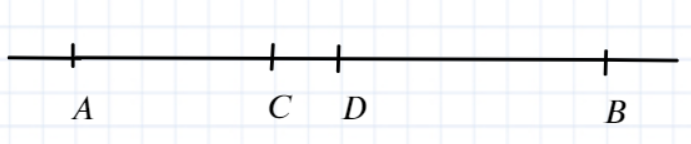
\includegraphics[scale=0.35]{qqqq.png}}
\end{figure}
\end{center}
150. Маленьких треугольников изображено 12, треугольников из 4 частей --- 5 и 1 самый большой. Всего треугольников $12+5+1=18.$\\
151. Перечислим все треугольники: ABF, BEC, BFC, BEK, KGC, KEC, GEC, FEG, ABC, FEC.\\
152. У 2017-го <<замечательного>> числа сумма цифр равна 2017. Число тем меньше, чем меньше количество его цифр, значит надо взять как можно больше цифр 9. Так как
$2017=9\cdot224+1,$ самое маленькое число, которое можно составить, равно $19\ldots9$(224 девятки).\\
153. Общая сторона у переднего и верхнего слоя должна быть равна 11 (общий делитель 44 и 77). Значит, изначально коробка имела размеры $4\times8\times11.$ После того, как съели передний слой, размеры стали $4\times7\times11,$ а после съедения верхнего --- $3\times7\times11.$ Таким образом, всего дети съедят $44+77+3\cdot7=142$ кусочка сахара, а изначально их было $4\cdot8\cdot11=352.$\\
154. Так как $176=16\cdot11,$ а $256=16\cdot16,$ ей следует купить пачки по 16 тетрадей (наибольший общий делитель чисел 176 и 256).\\
155. Подпишем все отрезки на картинке с учётом того, что правый верхний прямоугольник является квадратом.
\begin{center}
\begin{figure}[ht!]
\center{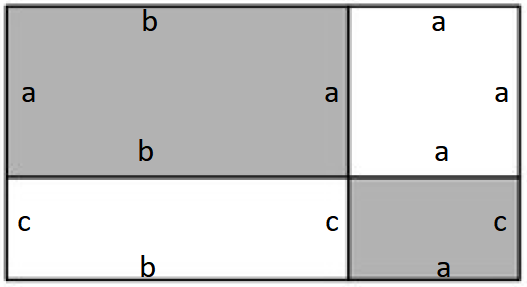
\includegraphics[scale=0.35]{37s.png}}
\end{figure}
\end{center}
Тогда $(a+b)\cdot2=34,\ a+b=17$см, $(a+c)\cdot2=22,\ a+c=11$см. Периметр всего прямоугольника равен $2\cdot(b+a+a+c)=2\cdot(17+11)=56$см. Его площадь равна $(b+a)(a+c)=17\cdot11=187\text{см}^2.$
ewpage
oindent
156. Расставим числа подбором:
\begin{center}
\begin{figure}[ht!]
\center{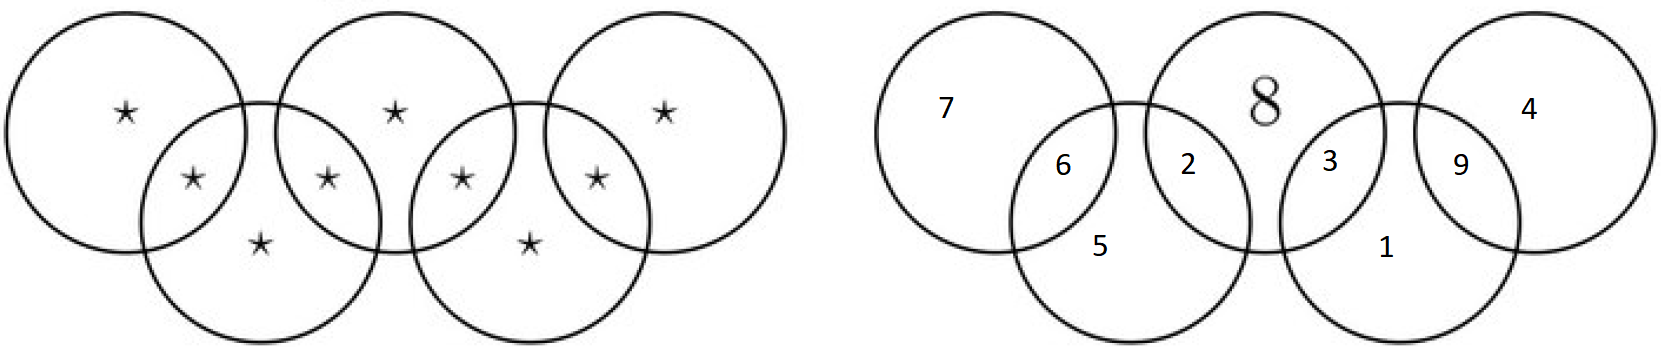
\includegraphics[scale=0.35]{38s.png}}
\end{figure}
\end{center}
157. В самом худшем случае нам никак не будет попадаться один из необходимых цветов и мы вытянем все $100+100+100=300$ остальных карандашей, кроме, например, красного. При вытягивании следующего, 301-го карандаша, мы точно получим желаемое.\\
158. Каждый город соединён с $9-1=8$ другими, поэтому авиалиний должно быть $9\cdot8=72.$ Но при таком подсчёте каждая авиалиния оказывается посчитана по 2 раза (как из $A$ в $B$ и как из $B$ в $A$), поэтому на самом деле их $72:2=36.$\\
159. Перечислим все 9 подходящих чисел: 30000, 21000, 20100, 20010, 20001, 12000, 10200, 10020, 10002.\\
160. Если у каждого мальчика есть сестра, мальчиков больше, чем девочек и бездетных семей нет, суммарно детей должно быть больше, чем взрослых.\\
161. Разница между первой и второй картинкой --- 1 среднее и 1 маленькое существо, значит их сумма равна $122-116=6$кг, поэтому большое существо весит $116-6=110$кг.\\
162. Так как Е оба раза не видно, она находится напротив одной из букв А, В, Г и напротив одной их букв Д, Б, В. Оба раза встречается только буква В, значит напротив неё и находится Е.\\
163. Подбором разделим фигуру на две одинаковые (как по размеру, так и по форме с учётом переворота) части:
\begin{center}
\begin{figure}[ht!]
\center{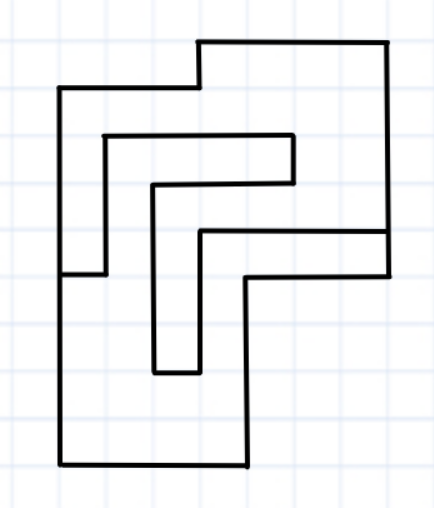
\includegraphics[scale=0.35]{9999.png}}
\end{figure}
\end{center}
164. Шариков не больше 11, иначе в 12 шариках не было бы ни одного кубика. Кубиков не больше 19, иначе в 20 кубиках не было бы ни одного шарика. Так как вместе их должно быть $30=11+19$ их должно быть ровно 11 и 19.\\
165. Подберём один из возможных вариантов:
\begin{center}
\begin{figure}[ht!]
\center{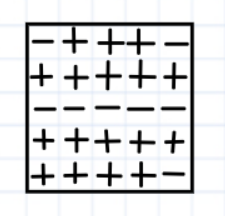
\includegraphics[scale=0.35]{31.png}}
\end{figure}
\end{center}
166. Понятно, что без переполнения это невозможно, значит надо подобрать число, кончающееся на много 9. Подходят числа 69999 и 70000.\\
167. Если это не так, они должны были бы собрать как минимум $0+1+2+3+\ldots+14=(1+14)+(2+13)+\ldots+(7+8)=7\cdot14=105$ компьютеров. Значит, какие-то двое точно собрали одинаковое число компьютеров.\\
168. Выпишем и сложим их все: $10+13+30+31=84.$\\
169. Найдём длины отрезков: $BL=32-28=4$см, $AL=32-22=10$см, тогда $KL=32-4-10=18$см.\\
170. Самой маленькой первой цифрой можно сделать 2, самой маленькой второй 4, значит надо зачеркнуть цифры 9, 5 и 7, получится число 24063.\\
171. Подбором найдём вариант $22\cdot2+22:2=55.$\\
172. Подбором найдём подходящую расстановку: а)$7200:(90-10)\cdot6=540,$ б) $8400:(3\cdot40)+20=90,$ в) $(210-30):(5\cdot3).$\\
173. Цифра 0 точно должна стоять в конце (других чётных цифр нет). Однозначное число одно: сам 0. Если число двузначное, то на первое место есть 3 варианта выбрать цифру. Если число трёхзначное, то на первое место 3 способа выбрать цифру, на второе уже 2, всего способов $3\cdot2=6.$ Если число четырёхзначное, то на первое место 3 способа выбрать цифру, на второе уже 2, а на третье --- 1, всего способов $3\cdot2\cdot1=6.$ Значит, всего чисел $1+3+6+6=16.$\\
174. На каждое место по 4 способа выбрать цифру, значит всего есть $4\cdot4\cdot=64$ числа.\\
175. В ближайшие сто лет --- значит до $2017+100=2117$ года. Первая цифра не поменяется, значит сумма 3 остальных должна быть равна $0+1+7=8.$ Перечислим все 9 подходящих чисел: $2026,\ 2035,\ 2044,\ 2053,$\\$2062,\ 2071,\ 2080,\ 2107,\ 2116.$\\
176. Каждый город соединён с $5-1=4$ другими, поэтому авиалиний должно быть $5\cdot4=20.$ Но при таком подсчёте каждая авиалиния оказывается посчитана по 2 раза (как из $A$ в $B$ и как из $B$ в $A$), поэтому на самом деле их $20:2=10.$\\
177. Если все надписи неправильные, бронзовая лампа не пуста и там не может жить злой джинн, значит в ней живёт добрый джинн.\\
178. Сергей не токарь, не электрик и не шофёр, значит он слесарь. Андрей не токарь и не электрик, значит он шофёр. Никита не слесарь, значит он электрик. Владимиру осталась профессия токаря.\\
179. Унесённые ёжиками грибы --- это унесённые мухоморы и унесённые белые. Мухоморы, которые сначала росли на полянке, --- это унесённые мухоморы и оставшиеся мухоморы. Первая часть у обоих количеств одинаковая, а вторые части равны по условию, значит унесённых грибов и изначально росших мухоморов поровну.\\
180. Коробочек с 5 шариками было 2, с 4 шариками --- $3-2=1,$ с 3 шариками --- $5-3=2,$ с 2 шариками --- $6-5=1,$ с 1 шариком --- $8-6=2.$ Значит, всего шариков было $5\cdot2+4\cdot1+3\cdot2+2\cdot1+1\cdot2=24.$\\
181. Пусть говорящих попугаев $x,$ тогда всего попугаев $7x,$ а говорящих животных --- $5x,$ значит попугаев больше.\\
182. В сапогах были $16-10=6$ мальчишек, кепку они также надели. Всего в кепке было $16-2=14$ мальчишек, значит $14-6=8$ были в кепке без сапог. Таким образом, мальчишек в кепке без сапог было на $8-6=2$ больше.\\
183. Девочки --- это босоногие девочки и обутые девочки. Босоногие дети --- это босоногие девочки и босоногие мальчики. Первая часть этих множеств совпадает, а вторые равны по условию, значит девочек столько же, сколько босоногих детей.\\
184. Если прав Шарик, то прав и Матроскин. Значит, Шарик ошибся, а Матроскин --- нет, поэтому дяд Фёдору больше 10 лет, но не больше 11. Значит, ему ровно 11 лет.\\
185. Все утверждения разные, значит верно ровно одно из них. Раз верно ровно одно, остальные 99 утверждений неверны. То есть верно утверждение <<В этой тетради ровно девяносто девять неверных утверждений>>.\\
186. Надо достать зерно из мешка с надписью <<Смесь>>. Если это мак, то в мешке лежит мак, в мешке с надписью <<Просо>> лежит смесь, а в мешке с надписью <<Мак>> --- просо. Случай, когда она достаёт просо, разбирается аналогично.\\
187. Пусть математиков-философов $x,$ тогда всего математиков $7x,$ а философов --- $9x,$ поэтому философов больше.\\
188. Если сложить периметры полученных прямоугольников, получится $320+410=730$см. Эта сумма больше периметра исходного прямоугольника, так как дополнительно 2 раза посчиталась их общая сторона, значит она равна $(730-536):2=97$см. Тогда вторая сторона у первого прямоугольника равна $320:2-97=63$см, а у второго --- $410:2-97=108$см. Таким образом меньше площадь первого прямоугольника и она равна $97\cdot63=6111\text{см}^2.$\\
189. Точка $K$ должна лежать на стороне $AB,$ точка $H$ на стороне $BC,$ точка $G$ на стороне $CD,$ а точка $E$ --- на стороне $AD.$ Тогда $(BK+BH)\cdot2=36$см, $(ED+GD)\cdot2=15$см, а значит $(BC+AD)\cdot2=(BH+HC+BK+KD)\cdot2=(BH+ED+BK+GD)\cdot2=(BH+BK)\cdot2+(ED+GD)\cdot2=36+15=51$см. С другой стороны, $(BC+AD)\cdot2=(AK+BK+AE+ED)\cdot2=(AK+AE)\cdot2+(BK+ED)\cdot2=29+(CG+HC)\cdot2,$ значит периметр $FHCG$ равен $51-29=22$см.\\
190. К периметру исходного прямоугольника добавятся 4 стороны приклеенных квадратов, поэтому их периметр также равен 52 см.\\
191. Обозначим буквами отрезки на картинке.
\begin{center}
\begin{figure}[ht!]
\center{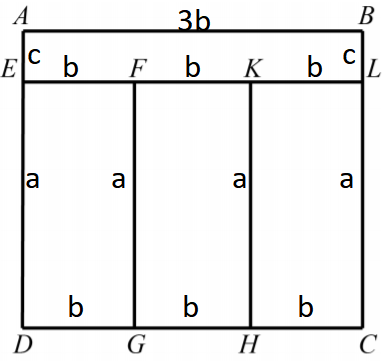
\includegraphics[scale=0.35]{41s.png}}
\end{figure}
\end{center}
Стороны, обозначенные буквой $a$ у прямоугольников одинаковые, периметры тоже, а поэтому одинаковы и стороны, обозначенные буквой $b.$ Тогда $3b=18,\ b=6$ см. Так как периметры одинаковы, имеем равенство $2\cdot(c+18)=2\cdot(6+a),\ c+18=6+16-c,\ 2c+18=22,\ c=2$см. Тогда у прямоугольника $ABLE$ стороны равны 2см и 18см, а у остальных прямоугольников --- 6см и $16-2=14$см.\\
192. Пусть школа построена на расстоянии $x$км от Орехово. Тогда суммарно школьники пройдут $300x+200(3-x)=300x+600-200x=100x+600.$ Это выражение минимально при $x=0,$ то есть когда школа построена в Орехово.\\
193. Пусть школа построена на расстоянии $x$км от А. Тогда суммарно школьники пройдут $100x+50(3-x)=100x+150-50x=50x+150.$ Это выражение минимально при $x=0,$ то есть когда школа построена в А.\\
194. Если мы вытащим два яблока, они могут быть разных цветов. Если вытащено 3 яблока, то у каких-то цвет должен совпасть, так как цветов всего два.\\
195. Если мы вытащим 6 яблок, то это могут быть по 2 яблока каждого цвета. Если вытащить 7 яблок, то у каких-то трёх цвет должен совпасть, иначе яблок максимум было бы $3\cdot2=6.$

Последнее красное яблоко может не попадаться нам до последнего, поэтому чтобы точно вытащить все красные яблоки, необходимо вытащить все 36 яблок

Какой-то из цветов может не попадаться нам до последнего, поэтому если мы вытащим 24 яблока, они могут быть только двух цветов. Если же мы вытащим 25 яблок, среди них точно будут все 3 цвета, иначе яблок было бы максимум $2\cdot12=24.$\\
196. Если бы пакетиков было 19 и меньше, их хватило бы максимум на $19\cdot3=57<58$ чашки чая. Если бы пакетиков было 21 и больше, их хватило бы минимум на $21\cdot2=42>41$ чашку чая. Значит, пакетиков было 20.\\
197. Пусть в этом числе содержится $a$ десятков и $b$ единиц (обратите внимание, что $a$ не обязательно является цифрой, например в числе 239 содержится 23 десятка). Тогда имеем равенство $10a+b=12a,\ 2a=b.$ Так как $b$ является цифрой, $a$ может принимать только значения от 1 до 4, поэтому исходное число могло быть равно 12, 24, 36, 48.\\
198. Если бы пакетиков в одной было 27 и меньше, их хватило бы максимум на $27\cdot3=81<83$ чашки чая. Если бы пакетиков в одной половине было 29 и больше, их хватило бы минимум на $29\cdot2=58>57$ чашек чая. Значит, пакетиков в одной половине было 28, а во всей коробке --- 56.\\
199. Пусть всего фруктов $x,$  тогда каждого вида по $x-2$ и $x=x-2+x-2+x-2,\ x=3x-6,\ 0=2x-6,\ 2x=6,\ x=3.$ Значит, всех фруктов было по $x-2=1.$\\
200. Груздей не больше 11 (иначе среди 12 груздей не найдётся рыжика), а рыжиков --- не больше 19 (иначе среди 20 рыжиков не найдётся груздя). Но так как $11+19=30$ а грибов всего 30, груздей должно быть ровно 11, а рыжиков --- 19.\\
201. а) Наименьшей первой цифрой можно сделать 1, получится число 18.\\
б) Наименьшей первой цифрой можно сделать 1, а второй --- 0, получится число 10.\\
202. Ровно 2 грани покрыты глазурью у кубиков, находящихся на ребре куба, кроме верхнего и нижнего. Если куб имел размеры $6\times6\times6,$ то как раз $6\cdot6\cdot6-4\cdot12=168.$ При меньших или больших размерах изначального куба останется меньше или больше кубиков соответственно. Значит, зайчата мальчики забрали $4\cdot12=48$ кубиков.\\
203. Всего кубиков получилось $5\cdot5\cdot5=125,$ а <<внутренних>> неокрашенных кубиков --- $3\cdot3\cdot3=27.$ Значит, кубиков с хотя бы одной окрашенной гранью было $125-27=98.$\\
204. Ровно три грани окрашены у тех кубиков, которые находятся в вершинах исходного куба. Их, как и вершин, 8.\\
205. Цикл начинается мизинцем и заканчивается безымянным пальцем, в нём 8 пальцев. Так как $2019:8=252$ (ост. 3), 2019-м будет третий палец в цикле, то есть средний.\\
206. Всего в считалочке 22 слова, так как $22:3=7$ (ост. 1), водить в любом случае будет Борис.\\
207. Последняя цифра будет изменяться по следующему правилу: $3,\ 9,\ 7,\ 1,\ 3\ldots$ В цикле 4 цифры, а $33:4=8$ (ост. 1), поэтому последней цифрой будет 3.\\
208. Один из людей может быть одновременно и сыном и отцом, то есть завтракали дедушка, его сын и его внук.\\
209. Это может быть, если профессор является женщиной.\\
210. Сестра является сестрой сразу для всех братьев, поэтому в семье $5+1=6$ детей.\\
211. В этой задаче ответ у каждого решающего свой.\\
212. Игра закончится ровно тогда, когда все кучки будут состоять из 1 камня. Для этого понадобится $10-1+15-1+20-1=42$ хода, значит выиграет второй. Заметим, что это игра-шутка: в ней нет никакой стратегии и второй выигрывает в любой случае.\\
213. Первому надо первым ходом взять 10 монет из первой кучки, после чего на столе останется две кучки по 20 монет. Теперь ему надо просто симметрично повторять ходы второго в другой кучке.\\
214. Второй может всегда повторять ходы первого в другой кучке (так как изначально кучки одинаковые).\\
215. Сделаем 1 взвешивание 2 монет. Если одна из монет легче, то она фальшивая, а если монеты равны, то фальшивой является оставшаяся монета.\\
216. Сначала разобьём монеты на 3 кучи по 9 монет. Взвесим 2 из них: если какая-то из куч легче, то фальшивая монета в ней, а если они равны, то в оставшейся куче. Кучу с фальшивой монетой разделим на 3 кучи по 3 монеты и взвесим 2 из них:  если какая-то из куч легче, то фальшивая монета в ней, а если они равны, то в оставшейся куче. Далее взвесим 2 монеты и найдём фальшивую (см. задачу 215).\\
217. Взвесим 2 монеты: если они равны, то фальшивая найдена. Если они не равны, то оставшаяся монета точно настоящая, взвесим её с одной из первых и найдём фальшивую. Итого понадобится 3 действия.

Взвесим 2 монеты: если они равны, то фальшивая среди оставшихся 2, а первые 2 монеты --- настоящие. Взвесим настоящую с одно из оставшихся: если они равны, то последняя монета --- фальшивая, в противном случае фальшивая взвешиваемая. Если первые 2 монеты не равны, то оставшиеся точно настоящие, взвесим одну из них с любой из первых 2 и аналогично найдём фальшивую. Итого понадобится 3 действия.

Разделим монеты на 3 группы по 3 монеты и взвесим 2 из них. Если они равны, то в последней группе все монеты настоящие. Взвесим её с одной из первых двух и определим, в какой группе фальшивая монета и легче она или тяжелее, далее действуем как в задаче 215. Если изначальные группы не равны, то в последней группе все монеты настоящие и взвесив её с одной из первых двух, найдём и группу с фальшивой монетой и определим, легче она или тяжелее. Далее действуем как в задаче 215. Итого понадобится 4 действия.\\
218. У человека 2 бабушки и 2 дедушки, 4 прабабушки и 4 прадедушки, 8 прапрабабушек и прапрадедушек. Значит, у наших прапрабабушек и прапрадедушек было $16cdot16=256$ прапрабабушек и прапрадедушек.\\
219. Пусть в этом числе было $x$ десятков, тогда $x=10x+4-229,\ 0=9x-225,\ 9x=225,\ x=25.$ Значит, это число 254.\\
220. Пусть в этом числе было $x$ десятков, тогда $x=10x-666,\ 0=9x-666,\ 9x=666,\ x=74.$ Значит, это число 740.\\
221. Всего кубиков было $6\cdot6\cdot6=216.$ Это количество равно двум у кубиков, идущих вдоль рёбер, кроме первого и последнего (у этих кубиков оно равно 3).
Таких кубиков $4\cdot12=48,$ значит не равно двум оно у $216-48=168$ кубиков.\\
222. Всего кубиков было $7\cdot7\cdot7=343.$ Это количество равно двум у кубиков, идущих вдоль рёбер, кроме первого и последнего (у этих кубиков оно равно 3).
Таких кубиков $5\cdot12=60,$ значит не равно двум оно у $343-60=283$ кубиков.\\
223. Подбором найдём один из возможных примеров.
\begin{center}
\begin{figure}[ht!]
\center{\includegraphics[scale=0.35]{166s.png}}
\end{figure}
\end{center}
224. Подбором найдём один из возможных примеров.
\begin{center}
\begin{figure}[ht!]
\center{\includegraphics[scale=0.35]{16s.png}}
\end{figure}
\end{center}
225. Подбором найдём подходящую картинку.
\begin{center}
\begin{figure}[ht!]
\center{\includegraphics[scale=0.35]{01s.png}}
\end{figure}
\end{center}
226. Гайки и молотки могут лежать только в ящике с надписью <<Отвёртки>>.\\
227. Наименьшее число, делящееся на 7, 35 и 42 --- это 210. Значит, напротив 7 стоит 30, напротив 35 стоит 6, а напротив 42 --- 5. Тогда сумма всех чисел равна $7+35+42+30+6+5=125.$\\
228. Число, которое не изменяется ни при каком умножении --- это 0, значит он стоит в разряде десятков. Самой большой первой цифрой можно взять 9, тогда самой большой второй цифрой будет 3, а третьей цифрой должна быть 6. Оставшиеся места заполним наибольшими из доступных цифр: 936807.\\
229. Число, которое не изменяется ни при каком умножении --- это 0, значит он стоит в разряде сотен. Самыми маленькими первыми двумя цифрами можно взять 1 и 2. Тогда самой маленькой тртьей цифро можно взять 6 (чтобы она делилась на 3), тогда пятой цифрой должна быть 9. Оставшиеся места заполним наименьшими из доступных цифр: 126093.\\
230. Перечислим все 15 чисел: 30000, 21000, 20100, 20010, 20001, 12000, 10200, 10020, 10002, 11100, 11010, 11001, 10110, 10101, 10011.\\
231. Перечислим все 20 чисел: 4000, 3100, 3010, 3001, 1300, 1030, 1003, 2200, 2020, 2002, 2011, 2101, 2110, 1201, 1210, 1102, 1120, 1012, 1021, 1111.\\
232. Подбором найдём один из возможных вариантов: 1212122122122.\\
233. Подбором найдём один из возможных вариантов: 1212122212122122121.\\
234. Если первый был рыцарем, то второй и третий --- лжецы. Но тогда второй сказал правду, чего быть не может. Значит, первый был лжецом. Если второй был рыцарем, то третий тоже был рыцарем, а значит сказал <<один>>. Если второй был лжецом, то третий тоже должен быть лжецом, но тогда первый сказал правду, чего быть не может. Значит, третий точно сказал <<один>>.\\
235. Если второй был рыцарем, то первый и третий --- лжецы. Но тогда первый сказал правду, чего быть не может. Значит, второй был лжецом. Если первый был рыцарем, то третий тоже был рыцарем, а значит сказал <<один>>. Если первый был лжецом, то третий тоже должен быть лжецом, но тогда второй сказал правду, чего быть не может. Значит, третий точно сказал <<один>>.\\
236. Приведём один из возможных примеров.
\begin{center}
\begin{figure}[ht!]
\center{\includegraphics[scale=0.3]{04.png}}
\end{figure}
\end{center}
237. Сверху вниз пирамида должна расширяться: от $1\times1$ до $4\times4.$ Чтобы построить ещё два уровня, понадобится $5\cdot5+6\cdot6=61$ кубик.\\
238. Днём это надпись верна с 14-00 до 23-00, то есть 9 часов. Ночью она верна столько же времени (с 2-00 до 11-00), а значит всего она верна $2\cdot9=18$часов.\\
239. Днём это надпись верна с 15-00 до 22-00, то есть 7 часов. Ночью она верна столько же времени (с 3-00 до 10-00), а значит всего она верна $2\cdot7=14$часов.\\
240. С помощью гирь 1кг и 2кг можно взвесить 1кг, 2кг и 3кг (если положить их на одну чашу). Если на первую чашу положить часть этих гирь, а на вторую --- 9кг, то можно также взвесить 6кг, 7кг и 8кг. И, наконец, если класть все гири (включая 9кг) на одну чашу, можно взвесить 9кг, 10кг, 11кг и 12кг.\\
241. С помощью гирь 1кг и 2кг можно взвесить 1кг, 2кг и 3кг (если положить их на одну чашу). Если на первую чашу положить часть этих гирь, а на вторую --- 10кг, то можно также взвесить 7кг, 8кг и 9кг. И, наконец, если класть все гири (включая 10кг) на одну чашу, можно взвесить 10кг, 11кг, 12кг и 13кг.\\
242. Если трёхзначными являются первые 2 числа (а последнее --- четырёхзначное), $N$ может принимать значения от 975 до 989 ($989-975+1=15$ чисел). Если трёхзначными являются последние два числа (а первое --- двузначное), то $N$ может принимать значения от 90 до 99 ($99-90+1=10$ чисел). Итого подходящих чисел $15+10=25.$\\
243. Если трёхзначными являются первые 2 числа (а последнее --- четырёхзначное), $N$ может принимать значения от 980 до 984 ($984-980+1=5$ чисел). Если трёхзначными являются последние два числа (а первое --- двузначное), то $N$ может принимать значения от 85 до 99 ($99-85+1=15$ чисел). Итого подходящих чисел $5+15=20.$\\
244. Палиндромы могут отличаться на 2 только при наличии переполнения во всех разрядах при переходе от меньшего к большему, это числа 9999 и 10001. Значит, искомое число равно $9999-3=9996.$\\
245. Палиндромы могут отличаться на 2 только при наличии переполнения во всех разрядах при переходе от меньшего к большему, это числа 9999 и 10001. Значит, искомое число равно $9999+5=10004.$\\
246. Удобнее считать, что если число сложить с его суммой цифр, получится 2019. Будем искать числа по отдельности в каждом десятке, так как внутри десятка при увеличении числа на 1 его сумма цифр также увеличивается на 1. Начнём с числа 2010: $2010+2+1=2013,$ на $2019-2013=6,$ значит необходимо увеличить число на $6:2=3.$ Число $2010+3=2013$ подходит: $2013+2+1+3=2019.$ В следующем десятке $2000+2=2002,$ отличается на $2019-2002=17,$ получить нужное число добавляя по 2 не получится. В следующем десятке $1990+1+9+9=2009,$ отличается на $2019-2009=10,$ значит необходимо увеличить число на $10:2=5.$ Число $1990+5=1995$ подходит: $1995+1+9+9+5=2019.$ В следующем десятке даже у самого большого числа слишком маленькая сумма: $1989+1+9+8+9=2016<2019,$ значит других ответов нет.\\
247. Удобнее считать, что если число сложить с его суммой цифр, получится 2021. Будем искать числа по отдельности в каждом десятке, так как внутри десятка при увеличении числа на 1 его сумма цифр также увеличивается на 1. Начнём с числа 2010: $2010+2+1=2013,$ на $2021-2013=8,$ значит необходимо увеличить число на $8:2=4.$ Число $2010+4=2014$ подходит: $2014+2+1+4=2021.$ В следующем десятке $2000+2=2002,$ отличается на $2021-2002=19,$ получить нужное число добавляя по 2 не получится. В следующем десятке $1990+1+9+9=2009,$ отличается на $2021-2009=12,$ значит необходимо увеличить число на $12:2=6.$ Число $1990+6=1996$ подходит: $1996+1+9+9+6=2021.$ В следующем десятке даже у самого большого числа слишком маленькая сумма: $1989+1+9+8+9=2016<2021,$ значит других ответов нет.\\
248. Самая маленькая возможная сумма 15 натуральных чисел равна $1+1+\ldots+1=15.$ Значит, надо увеличить её на $18-15=3,$ то есть к единицам каким-то образом добавить 3. Если добавить 3 к одной единице, произведение получится равно $1\cdot1\cdot\ldots\cdot1\cdot4=4.$ Если добавить к одной единице 1, а к другой 2, произведение получится равно $1\cdot1\cdot\ldots\cdot1\cdot2\cdot3=6.$ Если к трём единицам добавить по 1, произведение будет равно $1\cdot1\cdot\ldots\cdot1\cdot2\cdot2\cdot2=8.$ Значит, произведение могло быть равно 4, 6 или 8.\\
249. Самая маленькая возможная сумма 16 натуральных чисел равна $1+1+\ldots+1=16.$ Значит, надо увеличить её на $19-16=3,$ то есть к единицам каким-то образом добавить 3. Если добавить 3 к одной единице, произведение получится равно $1\cdot1\cdot\ldots\cdot1\cdot4=4.$ Если добавить к одной единице 1, а к другой 2, произведение получится равно $1\cdot1\cdot\ldots\cdot1\cdot2\cdot3=6.$ Если к трём единицам добавить по 1, произведение будет равно $1\cdot1\cdot\ldots\cdot1\cdot2\cdot2\cdot2=8.$ Значит, произведение могло быть равно 4, 6 или 8.\\
250. Вычтем по одной букве Б с обеих сторон, получим ДУБ+ДУБ+ДУ0=ББ0+36. Правая часть кончается на 6, значит Б+Б кончается на 6, поэтому Б может быть равно 3 или 8. В первом случае ДУБ$=(333+36):3=123,$ а во втором --- ДУБ$=(888+36):3=308.$\\
251. Вычтем по одной букве У с обеих сторон, получим МЯУ+МЯУ+МЯ0=УУ0+48. Правая часть кончается на 8, значит У+У кончается на 8, поэтому У может быть равно 4 или 9. В первом случае МЯУ$=(444+48):3=164,$ а во втором --- МЯУ$=(999+48):3=349.$\\
252. После того, как Дед Мороз закончит первый круг, он подарит $15\cdot1+15\cdot2=45$ подарков, по 2 подарка будет у 15 детей (у всех чётных номеров). У него останется $55-45=10$ подарков, значит он подарит ещё по 1 подарку детям с номерами 1, 3, 5 и 7 (у них станет по 2 подарка) и по 2 подарка детям с номерами 2, 4 и 6 (у них станет по 4 подарка). Тогда всего с 2 подарками окажется $15+4-3=16$ детей.\\
253. После того, как Дед Мороз закончит первый круг, он подарит $16\cdot2+16\cdot4=96$ подарков, по 4 подарка будет у 16 детей (у всех нечётных номеров). У него останется $112-96=16$ подарков, значит он подарит ещё по 4 подарка детям с номерами 1, 3, 5 (у них станет по 8 подарков) и по 2 подарка детям с номерами 2 и 4 (у них станет по 4 подарка). Тогда всего с 4 подарками окажется $16+2-3=15$ детей.\\
254. При удалении крайних клеток периметр полоски не поменяется, а при удалении соседних поменяется в сумме на 2, а должен на $48-(20+2)\cdot2=4.$ Значит, клетки необходимо удалять не крайние, не соседние и не приводящие к разваливанию полоски. Последовательно заполним полоску, написав в каждой клетке количество способов выбрать для неё вторую удаляемую клетку.
\begin{center}
\begin{figure}[ht!]
\center{\includegraphics[scale=0.3]{gg.png}}
\end{figure}
\end{center}
Так как крайние клетки брать нельзя, изначально для выбора остаётся $2\cdot20-4=36$ клеток. Вместе с левой верхней клеткой нельзя брать её саму и 3 её соседей, остаётся $36-4=32$ возможных клетки. Вместе со второй клеткой в верхнем ряду нельзя брать её саму и 5 соседей, остаётся $36-6=30$ возможных клеток. Далее у каждой следующей клетки будет на 1 вариант меньше (нельзя брать ранее рассмотренные клетки), пока мы не дойдём до последней клетки. Двумя её соседями являются изначально запрещённые крайние клетки, поэтому с ней можно брать $15-1+2=16$ клеток. Вместе с крайней левой клеткой нижней строки можно взять все клетки нижней строки кроме трёх с левого края и одной с правого, то есть опять $20-4=16$ клеток. Далее количество вариантов опять уменьшаться на 1, пока не дойдёт до 0. Значит, всего вариантов будет $32+30+29+28+\ldots+16+15+16+16+15+14+\ldots+2+1=1+2+\ldots+29+30+16+15+16+32=(1+30)+(2+29)+\ldots+(15+16)+79=31\cdot15+79=544.$
ewpage
oindent
255. При удалении крайних клеток периметр полоски не поменяется, а при удалении соседних поменяется в сумме на 2, а должен на $50-(21+2)\cdot2=4.$ Значит, клетки необходимо удалять не крайние, не соседние и не приводящие к разваливанию полоски. Последовательно заполним полоску, написав в каждой клетке количество способов выбрать для неё вторую удаляемую клетку.
\begin{center}
\begin{figure}[ht!]
\center{\includegraphics[scale=0.3]{gg1.png}}
\end{figure}
\end{center}
Так как крайние клетки брать нельзя, изначально для выбора остаётся $2\cdot21-4=38$ клеток. Вместе с левой верхней клеткой нельзя брать её саму и 3 её соседей, остаётся $38-4=34$ возможных клетки. Вместе со второй клеткой в верхнем ряду нельзя брать её саму и 5 соседей, остаётся $38-6=32$ возможные клетки. Далее у каждой следующей клетки будет на 1 вариант меньше (нельзя брать ранее рассмотренные клетки), пока мы не дойдём до последней клетки. Двумя её соседями являются изначально запрещённые крайние клетки, поэтому с ней можно брать $16-1+2=17$ клеток. Вместе с крайней левой клеткой нижней строки можно взять все клетки нижней строки кроме трёх с левого края и одной с правого, то есть опять $21-4=17$ клеток. Далее количество вариантов опять уменьшаться на 1, пока не дойдёт до 0. Значит, всего вариантов будет $34+32+31+30+\ldots+17+16+17+17+16+15+\ldots+2+1=1+2+\ldots+31+32+17+16+17+34=(1+32)+(2+21)+\ldots+(16+17)+84=33\cdot16+84=612.$\\
256. Сначала узнаем, сколько чисел у каждого из детей. Последняя цифра фиксирована, первую можно выбрать 9 способами (любая цифра кроме 0), вторую --- 10, значит всего чисел $9\cdot10=90.$ При этом каждое Анино число больше каждого Васиного с теми же первыми двумя цифрами на $9-8=1,$ а каждое Сашино больше Диминого на $4-2=2.$ Тогда Анина сумма больше Васиной на $90\cdot1=90,$ а Сашина больше Диминой на $90\cdot2=180.$ Поэтому у Ани и Саши сумма больше на $90+180=270.$\\
257. Сначала узнаем, сколько чисел у каждого из детей. Последняя цифра фиксирована, первую можно выбрать 9 способами (любая цифра кроме 0), вторую --- 10, значит всего чисел $9\cdot10=90.$ При этом каждое Анино число меньше каждого Васиного с теми же первыми двумя цифрами на $9-8=1,$ а каждое Сашино больше Диминого на $4-2=2.$ Тогда Анина сумма меньше Васиной на $90\cdot1=90,$ а Сашина больше Диминой на $90\cdot2=180.$ Поэтому у Ани и Саши сумма больше на $180-90=90.$\\
258. Самая большая сумма цифр будет у числа, содержащего наибольшее количество цифр 9. Это число 2699999.\\
259. Самая большая сумма цифр будет у числа, содержащего наибольшее количество цифр 9. Это число 3799999.\\
260. Нули на конце произведения получаются от умножения 5 на 2, так что возьмём в качестве первых двух слагаемых числа с наибольшим количеством пятёрок в множителях, это 25 и 50 (по 2). Тогда последнее число равно $83-25-50=8$ и $25\cdot50\cdot8=10000.$\\
261. Нули на конце произведения получаются от умножения 5 на 2, так что возьмём в качестве первых двух слагаемых числа с наибольшим количеством пятёрок в множителях, это 25 и 50 (по 2). Тогда последнее число равно $91-25-50=16$ и $25\cdot50\cdot16=20000.$\\
262. Очевидно, что если удалить одну клетку, прямоугольник на части не развалится. Удалить же две клетки можно следующим образом:
\begin{center}
\begin{figure}[ht!]
\center{\includegraphics[scale=0.3]{rus1.png}}
\end{figure}
\end{center}

ewpage
oindent
263. Очевидно, что если удалить одну клетку, прямоугольник на части не развалится. Удалить же две клетки можно следующим образом:
\begin{center}
\begin{figure}[ht!]
\center{\includegraphics[scale=0.3]{ris.png}}
\end{figure}
\end{center}
264. Если вычесть из 203 нечётную цифру (последняя цифра нечётного числа является нечётной), мы получим первые три цифры исходного числа. Нечётных цифр всего 5, разберём все варианты. Цифра 1: $203-1=202,$ исходное число $2021,$ цифра 3: $203-3=200,$ исходное число 2003, цифра 5: $203-5=198,$ исходное число 1985, цифра 7: $203-7=196,$ исходное число 1967, цифра 9: $203-9=194,$ исходное число 1949.\\
265. Если вычесть из 204 чётную цифру (последняя цифра чётного числа является чётной), мы получим первые три цифры исходного числа. Чётных цифр всего 5, разберём все варианты. Цифра 0: $204-0=204,$ исходное число $2040,$ цифра 2: $204-2=202,$ исходное число 2022, цифра 4: $204-4=200,$ исходное число 2004, цифра 6: $204-6=198,$ исходное число 1986, цифра 8: $204-8=196,$ исходное число 1968.\\
266. Выпишем первые 13 цифр: $1,\ 2,\ 2,\ 4,\ 8,\ 2,\ 6,\ 2,\ 2,\ 4,\ 8,\ 2,\ 6.$ Как мы видим, начиная со второй цифры последовательность зацикливается и цикл имеет длину 6. Остаток от деления $2021-1=2020$ на 6 равен 4, значит на 2021-м месте стоит четвёртое число из цикла, равное 8.\\
267. Выпишем первые 14 цифр: $2,\ 1,\ 2,\ 2,\ 4,\ 8,\ 2,\ 6,\ 2,\ 2,\ 4,\ 8,\ 2,\ 6.$ Как мы видим, начиная с третьей цифры последовательность зацикливается и цикл имеет длину 6. Остаток от деления $2021-2=2019$ на 6 равен 3, значит на 2021-м месте стоит третье число из цикла, равное 4.\\
268. Быстрее всего на табло окажутся 5 единиц в $11:14:11,$ это произойдёт через 38 секунд.\\
269. Быстрее всего на табло окажутся 5 единиц в $11:15:11,$ это произойдёт через 27 секунд.\\
270. Всего в прямоугольнике $100\times200$ было $100\cdot199+200\cdot99=39700$ перегородок (см. задачу 11 2017 года). Из-за дырок пропадут перегородки внутри них и их периметр, то есть $(7\cdot6+7\cdot6+7\cdot4)\cdot2=224$ перегородки. Останется $39700-224=39476$ перегородок.\\
271. Всего в прямоугольнике $100\times200$ было $100\cdot199+200\cdot99=39700$ перегородок (см. задачу 11 2017 года). Из-за дырок пропадут перегородки внутри них и их периметр, то есть $(8\cdot7+8\cdot7+8\cdot4)\cdot2=288$ перегородок. Останется $39700-288=39412$ перегородок.\\
272. Заметим, что кубик может попасть на ту же грань, на которой стоял, минимум через 3 перекатывания, значит испачкать можно максимум треть клеток, то есть $3\cdot5:3=5.$ На картинке приведён один из возможных вариантов это сделать. Испачканной выберем ту грань, которая стоит на клетках 2, 5, 8, 11, 14.
\begin{center}
\begin{figure}[ht!]
\center{\includegraphics[scale=0.35]{kub1s.png}}
\end{figure}
\end{center}

ewpage
oindent
273. Заметим, что кубик может попасть на ту же грань, на которой стоял, минимум через 3 перекатывания, значит испачкать можно максимум треть клеток, то есть $3\cdot6:3=6.$ На картинке приведён один из возможных вариантов это сделать. Испачканной выберем ту грань, которая стоит на клетках 2, 5, 8, 11, 14, 17.
\begin{center}
\begin{figure}[ht!]
\center{\includegraphics[scale=0.35]{kub2s.png}}
\end{figure}
\end{center}
274. Суммарно муравьишка проползёт 1 ребро <<к нам>>, одно ребро вниз, одно ребро вправо и одно ребро <<от нас>>, то есть $15\cdot4=60$ см.\\
275. Если провести вертикальную линию в середине данной фигуры, она распадётся на 4 треугольника. два верхних вместе составляют прямоугольник $1\times3,$ а два нижних --- $2\times4.$ Значит, всего в фигуре $1\cdot3+2\cdot4=11$ клеток.\\
276. Гречишный мёд не мог кончиться, так как $3>2.$ Липового мёда не могла стать меньше, чем гречишного, так как $6-3=3>2.$ Горшочков всех видов не могло стать поровну, так как даже липового и гречишного мёда не могла стать поровну. Если съеден 1 горшочек цветочного и 1 горшочек гречишного мёда, то цветочного и липового мёда станет поровну. Горшочков с цветочным мёдом 7, а всех остальных --- $6+3=9.$ Так как $9-2=7,$ горшочков с цветочным мёдом не может стать больше, чем остальных. Всего останется $7+6+3-2=14$ горшочков мёда. Если цветочный мёд не брать, то его останется ровно половина от общего количества. Таким образом, могли получится варианты 4 и 6.\\
277. Ровно три прямоугольника покрывают области 4, 7 и 9.\\
278. Средние весы находятся в равновесии. Если поменять местами треугольник и квадрат, то чаша с треугольником перевесит, значит треугольник тяжелее квадрата. Если поменять местами кружок и квадрат, то перевесит чаша с квадратом, значит кружок легче квадрата. Таким образом, самой лёгкой фигурой является кружок, а самой тяжёлой --- треугольник.\\
279. Подбором найдём подходящее число 8314.\\
280. Поворот налево (вместе со следующим движением) занимает у Феди $5+7=12$ секунд, а поворот направо --- $3+7=10$ секунд. Всё путешествие заняло $2\cdot60+2=122$ секунды. После первого поворота налево у Феди останется $122-12=110$ секунд, которые надо разбить на несколько слагаемых по 10 и по 12 секунд. Так как сумма заканчивается на 0, поворотов налево должно быть 0, 5, 10 и так далее. Если поворотов налево было 0, то поворотов направо было $110:10=11.$ Если поворотов налево было 5, то поворотов направо было $(110-5\cdot12):10=5.$ Больше поворотов быть не могло, так как $10\cdot12>110.$\\
281. Например, подходит число $4\cdot3\cdot5\cdot7=420.$\\
282. Например, подходит число $8\cdot9\cdot7=504.$\\
283. Например, подойдёт такая картинка:
\begin{center}
\begin{figure}[ht!]
\center{\includegraphics[scale=0.35]{pent.png}}
\end{figure}
\end{center}
ewpage

oindent284. Например, подойдёт такая картинка:
\begin{center}
\begin{figure}[ht!]
\center{\includegraphics[scale=0.35]{pant.png}}
\end{figure}
\end{center}
285. Он написал числа 16, 36, 56, 60, 64, 68, 76, и 96, в них 8 цифр 6.\\
286. Он написал числа 28, 48, 68, 80, 84 и 88, в них 7 цифр 8.\\
287. \begin{center}
\begin{figure}[ht!]
\center{\includegraphics[scale=0.35]{perim.png}}
\end{figure}
\end{center}
От периметра отнимется $6a,$ а добавится $2a,$ значит $6a-2a=4a=24,$ что и является периметром квадрата.\\
288. \begin{center}
\begin{figure}[ht!]
\center{\includegraphics[scale=0.35]{perim.png}}
\end{figure}
\end{center}
От периметра отнимется $6a,$ а добавится $2a,$ значит $6a-2a=4a=36,$ что и является периметром квадрата.\\
289. Такие дни есть в каждом месяце, кроме ноября и декабря, так как $3\cdot11=33>30,$ значит их 10.\\
290. Такие дни есть только в первых 7 месяцах, так как $8\cdot4=32>31,$ значит их 7.\\
291. В ПН с ПТ и ВТ с СБ он назовёт две пары одинаковых чисел. В СР, ЧТ и ВС он также должен назвать 3 одинаковых числа, при этом называемые в этих трёх случаях числа различны. Значит, три числа 3 --- это СР, ЧТ и ВС, а поэтому Саша родился 4 числа. Но тогда в остальные дни он должен был говорить 12 и 4, а этих чисел среди его ответов нет.\\
292. Подберём, например, $951+834+762=2547.$\\
293. Подберём, например, $951+832+760=2543.$\\
294. Всего пятизначных чисел $99999-10000+1=90000.$ Посчитаем количество чисел, в которых нет цифр 5 или 7. На первое место можно поставить 7 цифр (без 5, 7 и 0), а на все остальные места --- по 8 (без 5 и 7), значит всего таких чисел $7\cdot8\cdot8\cdot8\cdot8=28672.$ Тогда количество чисел, в записи каждого из которых есть цифра 5 или цифра 7, равно $90000-28672=61328.$\\
295. Всего пятизначных чисел $99999-10000+1=90000.$ Посчитаем количество чисел, в которых нет цифр 2 или 4. На первое место можно поставить 7 цифр (без 2, 4 и 0), а на все остальные места --- по 8 (без 2 и 4), значит всего таких чисел $7\cdot8\cdot8\cdot8\cdot8=28672.$ Тогда количество чисел, в записи каждого из которых есть цифра 2 или цифра 4, равно $90000-28672=61328.$\\
296. Число, полученное из исходного вычёркиванием предпоследней цифры, кончается на ту же цифру, что и исходное. Раз сумма кончается на 4, последняя цифра исходного числа могла быть 2 или 7. В первом случае число, полученное из исходного вычёркиванием предпоследней цифры, равно $204-2=202,$ то есть исходное число равно $\overline{20x2}$ и максимальная сумма цифр такого числа равна $2+0+9+2=13.$ Во втором случае число, полученное из исходного вычёркиванием предпоследней цифры, равно $204-7=197,$ то есть исходное число равно $\overline{19x7}$ и максимальная сумма цифр такого числа равна $1+9+9+7=26,$ таким образом ответом является число 1997.\\
297. Число, полученное из исходного вычёркиванием предпоследней цифры, кончается на ту же цифру, что и исходное. Раз сумма кончается на 6, последняя цифра исходного числа могла быть 3 или 8. В первом случае число, полученное из исходного вычёркиванием предпоследней цифры, равно $206-3=203,$ то есть исходное число равно $\overline{20x3}$ и максимальная сумма цифр такого числа равна $2+0+9+3=14.$ Во втором случае число, полученное из исходного вычёркиванием предпоследней цифры, равно $206-8=198,$ то есть исходное число равно $\overline{19x8}$ и максимальная сумма цифр такого числа равна $1+9+9+8=27,$ таким образом ответом является число 1998.\\
298. Последний раз пять из шести цифр на табло часов были одинаковыми в $11:21:11,$ то есть 8 минут и 49 секунд назад.\\
299. Последний раз пять из шести цифр на табло часов были одинаковыми в $22:32:22,$ то есть 7 минут и 38 секунд назад.\\
300. Если сторона квадрата равна $x,$ то в нём $x(x-1)+(x-1)x=2x(x-1)$ внутренних перегородок. При вырезании дырки $2\times2$ пропадают 4 перегородки внутри неё и $2\cdot4=8$ перегородок на её периметре. Значит, до вырезания квадратов перегородок было $20952+5\cdot(4+8)=21012$ и $2x(x-1)=21012,\ x(x-1)=10506.$ Так как это количество близко к 10000, сторона квадрата немногим больше 100. Подбором найдём $x=103.$\\
301. Если сторона квадрата равна $x,$ то в нём $x(x-1)+(x-1)x=2x(x-1)$ внутренних перегородок. При вырезании дырки $2\times2$ пропадают 4 перегородки внутри неё и $2\cdot4=8$ перегородок на её периметре. Значит, до вырезания квадратов перегородок было $21364+5\cdot(4+8)=21424$ и $2x(x-1)=21424,\ x(x-1)=10712.$ Так как это количество близко к 10000, сторона квадрата немногим больше 100. Подбором найдём $x=104.$\\
302. Пусть четвероклассников было $x,$ тогда пятиклассников было  $50-x.$ Посчитаем рукопожатия между четвероклассниками и пятиклассниками: с одной стороны их $4x,$ а с другой --- $6\cdot(50-x).$ Тогда $4x=6\cdot(50-x),\
4x=300-6x,\ 10x=300,\ x=30.$\\
303. Пусть пятиклассников было $x,$ тогда четвероклассников было  $50-x.$ Посчитаем рукопожатия между четвероклассниками и пятиклассниками: с одной стороны их $7x,$ а с другой --- $3\cdot(50-x).$ Тогда $7x=3\cdot(50-x),\
7x=150-3x,\ 10x=150,\ x=15.$ Заметим, что такая ситуация невозможна: для того, чтобы посчитать количество рукопожатий между пятиклассниками, необходимо 15 умножить на 5 и разделить на 2 (каждое рукопожатие окажется посчитано 2 раза). Но тогда количество рукопожатий окажется нецелым, что невозможно.\\
304. Например, можно расставить так:
\begin{figure}[ht!]
\center{\includegraphics[scale=0.35]{SUH.png}}
\end{figure}\\
305. Например, можно расставить так:
\begin{figure}[ht!]
\center{\includegraphics[scale=0.35]{PRAT.png}}
\end{figure}\\
306. Сначала найдём сторону маленьких квадратиков, она равна $100:5=20$см. Если кубик поставить на заднюю грань, то в него можно будет налить $100\cdot100\cdot60=600000\text{ см}^3=600\text{ дм}^3=600$л. В других случаях объём воды будет меньше, так как основание всегда равно $100\text{ см}\times100\text{ см},$ а высота 60 см при таком расположении дырок максимальна.\\
307. Сначала найдём сторону маленьких квадратиков, она равна $100:5=20$см. Если кубик поставить на заднюю грань, то в него можно будет налить $100\cdot100\cdot80=800000\text{ см}^3=800\text{ дм}^3=800$л. В других случаях объём воды будет меньше, так как основание всегда равно $100\text{ см}\times100\text{ см},$ а высота 80 см при таком расположении дырок максимальна.\\
308. На глаз определим: 321.\\
309. На глаз определим: 213.\\
310. Раз все надписи ложны, в банке с надписью <<Горох или пуговицы>> может лежать только мука.\\
311. Раз все надписи ложны, в банке с надписью <<Крупа или гайки>> может лежать только сахар.\\
312.\begin{figure}[ht!]
\center{\includegraphics[scale=0.35]{otr1.png}}
\end{figure}\\
Найдём $AC=AB-BC=10-3=7$см, $BK=CK-BC=8-3=5$см, тогда $AK=AC+BC+BK=7+3+5=15$см.\\
313. \begin{figure}[ht!]
\center{\includegraphics[scale=0.35]{otr2.png}}
\end{figure}\\
Найдём $MK=MP-PK=12-2=10$см, $PA=KA-PK=6-2=4$см, тогда $AM=MK+KP+PA=10+2+4=16$см.\\
314. Чтобы число было чётным, необходимо вычеркнуть 1, наибольшей первой цифрой можно сделать 9 (вычеркнуть 2), наибольшей второй --- 5, а наибольшей третьей --- 6 (вычеркнуть 4). Таким образом, получим число 95638.\\
315. Чтобы число было нечётным, необходимо вычеркнуть 8, наименьшей первой цифрой можно сделать 2, а наименьшей второй --- 4 (вычеркнуть 9 и 5). Таким образом, получим число 24631.\\
316. Сторона маленького квадрата равна 8 см (так как $8\cdot8=64$). Тогда сторона большого квадрата равна $8+8=16$см, а сторона среднего квадрата --- $(8+16):2=12$см. Тогда стороны самого большого прямоугольника равны $2\cdot12=24$см и $12+16=28$см, а значит его периметр равен $(24+28)\cdot2=104$см.\\
317. Сторона маленького квадрата равна 4 см (так как $4\cdot4=16$). Тогда сторона большого квадрата равна $4+4=8$см, а сторона среднего квадрата --- $(4+8):2=6$см. Тогда стороны самого большого прямоугольника равны $2\cdot6=12$см и $6+8=14$см, а значит его периметр равен $(12+14)\cdot2=52$см.\\
318. Если никто не получил чего-то больше, чем другой, все получили одинаковое количество конфет и одинаковое количество бутербродов. Но тогда и количество конфет $472=8\cdot59$ делится на общее количество людей, и количество бутербродов $118=2\cdot59$ также на него делится. Но тогда общее количество людей может быть равно только 59 (так как $35\cdot2<118).$ Число 59 можно представить в виде суммы двух слагаемых, отличающихся не более, чем на два только как $29+30,$ значит в меньшей группе было 29 человек.\\
319. Если никто не получил чего-то больше, чем другой, все получили одинаковое количество конфет и одинаковое количество бутербродов. Но тогда и количество конфет $427=7\cdot61$ делится на общее количество людей, и количество бутербродов $122=2\cdot61$ также на него делится. Но тогда общее количество людей может быть равно только 61.  Число 61 можно представить в виде суммы двух слагаемых, отличающихся не более, чем на два только как $31+30,$ значит в большей группе был 31 человек.\\
320. Подбором найдём $82+93=175.$\\
321. Подбором найдём $84+92=176.$\\
322. Максимальное пересечение реализуется на нижеприведённой картинке и его длина равна 5 см.\\
\begin{figure}[ht!]
\center{\includegraphics[scale=0.35]{lom1.png}}
\end{figure}\\
323. Максимальное пересечение реализуется на нижеприведённой картинке и его длина равна 10 см.\\
\begin{figure}[ht!]
\center{\includegraphics[scale=0.35]{lom1.png}}
\end{figure}\\
324. Выбирая каждый раз карточки так, чтобы сделать следующую цифру наименьшей, получим число 19341415778.\\
325. Выбирая каждый раз карточки так, чтобы сделать следующую цифру наименьшей, получим число 13343435747.\\
326. Расстояние между серединами крайних отрезков --- это разность между длиной всего отрезка и суммой половинок крайних отрезков. Значит, сумма половинок крайних отрезков равна $28-16=12$см, а тогда средний отрезок равен $16-12=4$см.\\
327. Расстояние между серединами крайних отрезков --- это разность между длиной всего отрезка и суммой половинок крайних отрезков. Значит, сумма половинок крайних отрезков равна $30-16=14$см, а тогда средний отрезок равен $16-14=2$см.\\
328. \begin{figure}[ht!]
\center{\includegraphics[scale=0.35]{sco1.png}}
\end{figure}\\
329. \begin{figure}[ht!]
\center{\includegraphics[scale=0.35]{sco2.png}}
\end{figure}\\
330. Произведя вычитание в столбик, найдём эту разность: $\underbrace{99\ldots99}_{2018}7978.$ Её сумма цифр равна $9\cdot2018+7+9+7+8=18193.$\\
331. Произведя вычитание в столбик, найдём эту разность: $\underbrace{99\ldots99}_{2017}7979.$ Её сумма цифр равна $9\cdot2017+7+9+7+9=18185.$\\
332. Петины числа: $6,\ 12,\ 18,\ \ldots$ Васины числа: $3,\ 9,\ 15,\ \ldots$ Каждое Петино число больше соответствующего Васиного на 3, значит разность их сумм равна $1000\cdot3=3000.$\\
333. Петины числа: $10,\ 20,\ 30,\ \ldots$ Васины числа: $5,\ 15,\ 25,\ \ldots$ Каждое Петино число больше соответствующего Васиного на 5, значит разность их сумм равна $1000\cdot5=5000.$\\
334. К моменту своей первой встречи Крош и Бараш совместно прошли расстояние между их домами, потратив на это 30 минут. К моменту своей второй встречи они совместно пройдут 3 расстояния между их домами, значит потратят на это $3\cdot30=90$ минут и встретятся в $10:30.$\\
335. К моменту своей первой встречи Крош и Бараш совместно прошли расстояние между их домами, потратив на это 60 минут. К моменту своей второй встречи они совместно пройдут 3 расстояния между их домами, значит потратят на это $3\cdot60=180$ минут и встретятся в $13:00.$\\
336. Если первая и последняя цифры Петиного числа равны, то их разница не будет трёхзначной. Значит, его первая цифра больше последней. Но тогда если записать вычитание этих чисел столбиком, в разряде десятков будут стоять одинаковые цифры, а для разряда единиц из этого разряда придётся занимать. Тогда надо занимать и из разряда сотен, а в разряде десятков будет $x+10-1-x=9.$\\
337. Посмотрим на разряд сотен. Так как $4+2=6,$ а в результате в разряде сотен стоит 7, сумма двузначных чисел, которыми кончаются слагаемые, равна 193. Это могут быть числа 99 и 94, 98 и 95 или 97 и 96. Сумма их цифр в любом случае равна 31. Так как $5+8=13,$ в разряде тысяч у суммы в любом случае стоит цифра 3. Так как сумма начинается с 10, сумма цифр, стоящих в разряде сотен тысяч должна быть равна 9. Значит, сумма всех цифр, заменённых звёздочками, равна $31+3+9=43.$\\
338. Посмотрим на разряд сотен. Так как $2+3=5,$ а в результате в разряде сотен стоит 6, сумма двузначных чисел, которыми кончаются слагаемые, равна 191. Это могут быть числа 99 и 92, 98 и 93, 97 и 94 или 96 и 95. Сумма их цифр в любом случае равна 29. Так как $6+7=13,$ в разряде тысяч у суммы в любом случае стоит цифра 3. Так как сумма начинается с 11, сумма цифр, стоящих в разряде сотен тысяч должна быть равна 10. Значит, сумма всех цифр, заменённых звёздочками, равна $29+3+10=42.$\\
339. Пусть все три числа кончаются на двузначное число $x.$ Тогда $x+x+x=3x=...17.$ Подходит окончание 117, тогда $x=117:3=39.$ Подбором найдём первые цифры: $139+239+439=817.$\\
340. Пусть все три числа кончаются на двузначное число $x.$ Тогда $x+x+x=3x=...17.$ Подходит окончание 117, тогда $x=117:3=39.$ Подбором найдём первые цифры: $139+239+539=917.$\\
341. Если первая цифра равна 1, то третья цифра может быть только 0. Если она равна 2, то третья цифра может быть равна 0 или 1. И так далее, для первой цифры 9 будет 9 вариантов третьей цифры (от 0 до 8). Значит, количество способов выбрать первую и третью цифры равно $1+2+\ldots+9=45.$ В каждом из вариантов оставшиеся 3 цифры могут быть любыми от 0 до 9, значит всего таких чисел $45\cdot10\cdot10\cdot10=45000.$\\
342. Если первая цифра равна 1, то четвёртая цифра может быть только 0. Если она равна 2, то четвёртая цифра может быть равна 0 или 1. И так далее, для первой цифры 9 будет 9 вариантов четвёртой цифры (от 0 до 8). Значит, количество способов выбрать первую и четвёртую цифры равно $1+2+\ldots+9=45.$ В каждом из вариантов оставшиеся 3 цифры могут быть любыми от 0 до 9, значит всего таких чисел $45\cdot10\cdot10\cdot10=45000.$
ewpage
oindent
343. \begin{figure}[ht!]
\center{\includegraphics[scale=0.35]{murav.png}}
\end{figure}\\
Чтобы добраться из точки $A$ до точки $B$ и из точки $E$ до точки $F,$ жуку надо сделать по $(2025-7):2-1=1008$ шагов. Чтобы добраться от точки $B$ до точки $C$ и от точки $D$ до точки $E$ ему понадобится по 7 шагов. Чтобы добраться от точки $C$ до точки $D$ ему понадобится 1 шаг. Значит, всего ему надо сделать $1008\cdot2+7\cdot2+1=2031$ шаг.\\
344. \begin{figure}[ht!]
\center{\includegraphics[scale=0.35]{murav.png}}
\end{figure}\\
Чтобы добраться из точки $A$ до точки $B$ и из точки $E$ до точки $F,$ жуку надо сделать по $(2023-7):2-1=1007$ шагов. Чтобы добраться от точки $B$ до точки $C$ и от точки $D$ до точки $E$ ему понадобится по 7 шагов. Чтобы добраться от точки $C$ до точки $D$ ему понадобится 1 шаг. Значит, всего ему надо сделать $1007\cdot2+7\cdot2+1=2029$ шагов.\\
345. Все числа в таблице, кроме 1, являются чётными. Значит, чтобы собрать ровно 25 цветков, необходимо сначала дойти до клетки с 1 цветком, а потом из неё попасть в правую верхнюю клетку. Путей из 1 в правую верхнюю клетку существует 3, и на каждом из них Вася соберёт $2+4+4=10$ цветков. Значит, на пути из левой нижней клетки до 1 Вася должен собрать $25-10-1=14$ цветков. Это можно сделать двумя способами, собрав $8+4+2=14$ цветков. Таким образом, всего подходящих маршрутов $3\cdot2=6.$\\
346. Все числа в таблице, кроме 7, являются чётными. Значит, чтобы собрать ровно 43 цветка, необходимо сначала дойти до клетки с 7 цветками, а потом из неё попасть в правую верхнюю клетку. Путей из 7 в правую верхнюю клетку существует 3, и на каждом из них Вася соберёт $8+6+6=20$ цветков. Значит, на пути из левой нижней клетки до 7 Вася должен собрать $43-20-7=16$ цветков. Это можно сделать двумя способами, собрав $2+6+8=16$ цветков. Таким образом, всего подходящих маршрутов $3\cdot2=6.$\\
347. В первый раз все цифры будут различными в $23:40:15,$ второй раз в $23:40:16,$ третий раз в $23:40:17,$ четвёртый раз в $23:40:18,$ пятый раз в $23:40:19,$ шестой раз в $23:40:51.$\\
348. В первый раз все цифры будут различными в $12:30:45,$ второй раз в $12:30:46,$ третий раз в $12:30:47,$ четвёртый раз в $12:30:48,$ пятый раз в $12:30:49,$ шестой раз в $12:30:54,$ в седьмой раз в $12:30:56.$\\
349. Раз Виктор проиграл Георгию четверть игр между ними, всего было 4 игры, 3 из которых он выиграл, то есть игры Виктора и Георгия закончились со счётом $3:1,$ а Георгия и Виктора --- $1:3.$ Алексей проиграл Борису 2 раза, значит и всем остальным он проиграл по 2 раза, и игры Виктора и Алексея закончились со счётом $2:3,$ Алексея и Виктора $3:2,$ Алексея и Бориса $1:2,$ Бориса и Алексея $2:1.$ Из таблицы определим, что Георгий проиграл Борису 2 раза, а выиграл у него 0 раз, значит игры Бориса и Георгия закончились со счётом $2:0,$ а Георгия и Бориса со счётом $0:2.$ Борис выиграл 5 раз, значит игры Бориса и Виктора закончились со счётом $1:7,$ а Виктора и Бориса --- $7:1.$ Георгий выиграл 3 раза, значит проиграл он 9 раз, и игры Алексея и Георгия закончились со счётом $4:2,$ а Георгия и Алексея --- $2:4.$ Таким образом, таблица полностью заполнена.
\begin{figure}[ht!]
\center{\includegraphics[scale=0.35]{tab2.png}}
\end{figure}\\
350. Раз Георгий проиграл Дмитрию треть игр между ними, всего было 3 игры, 2 из которых он выиграл, то есть игры Георгия и Дмитрия закончились со счётом $2:1,$ а Дмитрия и Георгия --- $1:2.$ Борис проиграл Виктору 3 раза, значит и всем остальным он проиграл по 3 раза, и игры Бориса и Виктора закончились со счётом $1:3,$ Виктора и Бориса $3:1,$ Георгия и Бориса $3:3,$ Бориса и Георгия $3:3.$ Из таблицы определим, что Дмитрий проиграл Виктору 2 раза, а выиграл у него 0 раз, значит игры Виктора и Дмитрия закончились со счётом $2:0,$ а Дмитрия и Виктора со счётом $0:2.$ Виктор выиграл 5 раз, значит игры Виктора и Георгия закончились со счётом $0:7,$ а Георгия и Виктора --- $7:0.$ Дмитрий выиграл 4 раза, значит проиграл он 12 раз, и игры Бориса и Дмитрия закончились со счётом $8:3,$ а Дмитрия и Бориса --- $3:8.$ Таким образом, таблица полностью заполнена.\\
\begin{figure}[ht!]
\center{\includegraphics[scale=0.35]{tab1.png}}
\end{figure}\\
351. Ближайшее к 2002 такое число --- 1991.\\
352. Ближайшее к 3003 такое число --- 2992.\\
353. \begin{figure}[ht!]
\center{\includegraphics[scale=0.35]{kovr1.png}}
\end{figure}\\
Наименьшая площадь будет покрыта сразу двумя коврами в том случае, когда они лежат в противоположных углах комнаты. В этом случае они вместе покрывают квадрат размером $9\times9$ метров, его площадь равна $9\cdot9=81\text{ м}^2.$
ewpage
oindent
354. \begin{figure}[ht!]
\center{\includegraphics[scale=0.35]{kovr1.png}}
\end{figure}\\
Наименьшая площадь будет покрыта сразу двумя коврами в том случае, когда они лежат в противоположных углах комнаты. В этом случае они вместе покрывают квадрат размером $10\times10$ метров, его площадь равна $10\cdot10=100\text{ м}^2.$\\
355. Самой большой первой цифрой может быть 9, тогда самой большой второй --- 7, третьей --- 5, а четвёртой --- 8, и так далее. Выбирая каждый раз самую большую возможную цифру, получим 9758642031.\\
356. Самой маленькой первой цифрой может быть 1, тогда самой маленькой второй --- 3, третьей --- 0, а четвёртой --- 2, и так далее. Выбирая каждый раз самую маленькую возможную цифру, получим 1302468579.\\
357. Всего шариков $4+7+8+10+11=40,$ значит всех должно стать по $40:5=8.$ Поэтому надо перекрасить как минимум 2 белых и 3 чёрных, то есть $2+3=5$ шариков. Если перекрасить чёрный шарик в зелёный, а потом по 2 белых и чёрных в красные, то всех шариков станет поровну.\\
358. Всего шариков $3+7+9+10+11=40,$ значит всех должно стать по $40:5=8.$ Поэтому надо перекрасить как минимум 1 синий, 2 белых и 3 чёрных, то есть $1+2+3=6$ шариков. Если перекрасить синий шарик в зелёный, а потом 2 белых и 3 чёрных в красные, то всех шариков станет поровну.\\
359. Можно зачеркнуть 3 и 2, тогда $6/1+5=84/12+4$, 8 и 2, тогда $36/12+5=4/1+4,$ 4 и 1, тогда $36/12+5=8/2+4.$\\
360. Можно зачеркнуть 4 и 2, тогда $8/1+3=72/12+5$, 7 и 2, тогда $48/12+3=2/1+5.$\\
361. $\underbrace{99\ldots99}_{100}+2023=1\underbrace{00\ldots00}_{100}-1+2023=1\underbrace{00\ldots00}_{96}2022.$ Сумма цифр этого числа равна $1+2\cdot3=7.$\\
362. $\underbrace{99\ldots99}_{100}+2024=1\underbrace{00\ldots00}_{100}-1+2024=1\underbrace{00\ldots00}_{96}2023.$ Сумма цифр этого числа равна $1+2\cdot2+3=8.$\\
363. Представим, что каждый раз за победу в партии каждой победительнице выдавали по медали. Тогда всего было выдано $6\cdot2=12$ медалей, значит Даша получила $12-5-2-1=4$ из них, то есть 4 раза была в команде-победительнице.\\
364. Представим, что каждый раз за победу в партии каждой победительнице выдавали по медали. Тогда всего было выдано $6\cdot2=12$ медалей, значит Даша получила $12-4-3-2=3$ из них, то есть 3 раза была в команде-победительнице.\\
365. Стараясь делать идущие раньше цифры как можно больше, найдём число 9860725.\\
366. Стараясь делать идущие раньше цифры как можно меньше, найдём число 1203794.\\
367. В двух трёхзначных числах 6 цифр, раз повторяется только одна, значит точно использован 0, поэтому произведение всех этих цифр равно 0. Тогда сумма равна $99+0=99.$\\
368. В двух трёхзначных числах 6 цифр, раз повторяется только одна, значит точно использован 0, поэтому произведение всех этих цифр равно 0. Тогда разность равна $100-0=100.$\\
369. Он не выполнит обещание только в том случае, если не сделает ничего из обещанного, поэтому правильный ответ Б.\\
370. Она не выполнит обещание только в том случае, если не сделает ничего из обещанного, поэтому правильный ответ В.\\
371. Этот шифр устроен так: в верхнем правом квадранте указывается число единиц, в верхнем левом квадранте --- число десятков,
в нижнем правом квадранте --- число сотен, в нижнем левом квадранте --- число тысяч. Значит, изображено число 486.\\
372. Этот шифр устроен так: в верхнем правом квадранте указывается число единиц, в верхнем левом квадранте --- число десятков,
в нижнем правом квадранте --- число сотен, в нижнем левом квадранте --- число тысяч. Значит, изображено число 175.\\
373. Чтобы число делилось на 2 и на 5, достаточно, чтобы оно оканчивалось на 0. Наибольшее подходящее число, оканчивающееся на 0 --- это 6320.\\
374. Чтобы число делилось на 2 и на 5, достаточно, чтобы оно оканчивалось на 0. Наибольшее подходящее число, оканчивающееся на 0 --- это 7240.\\
375. Нужно перевернуть монеты с изображением 1, 5 и короны. На остальных монетах либо точно другой рисунок, либо точно другое число.\\
376. Нужно перевернуть монеты с изображением 5, 10 и замка. На остальных монетах либо точно другой рисунок, либо точно другое число.\\
377. Добраться до первой точки на горизонтальной прямой от начала до конца до второй --- 4 варианта (через верх, через низ или со сменой верха на низ или низа на верх). От второй до третьей --- 3 варианта. От третьей до конца --- также 4. Значит, всего способов $4\cdot3\cdot4=48.$\\
378. Он мог сделать это, например, так:
\begin{figure}[ht!]
\center{\includegraphics[scale=0.35]{ums1.png}}
\end{figure}\\
379. Он мог сделать это, например, так:
\begin{figure}[ht!]
\center{\includegraphics[scale=0.35]{ums2.png}}
\end{figure}\\
380. Из условия следует, что пятая цифра всегда должна быть равна 2, тогда и седьмая тоже равна 2. Переберём все возможные четвёртые цифры: 06012021 (06 не двузначное), 11022022 (подходит), 16032023 (подходит), 21042024 (подходит), 26052025 (подходит), 31062026 (31.06 не бывает), 36072027, 41082028, 46092029 (чисел 36, 41 и 46 не существует). Значит, подходят 4 даты.\\
381. Заметим, что при каждом действии чётность перемещений фишки вправо и вверх одинакова. Но Матвею суммарно необходимо подвинуть фишку на 35 вправо и на 38 вверх, значит он этого сделать не сможет.\\
382. Заметим, что при каждом действии чётность перемещений фишки влево и вверх одинакова. Но Матвею суммарно необходимо подвинуть фишку на 37 влево и на 34 вверх, значит он этого сделать не сможет.\\
383. Подбором найдём пример: $239+681=920.$\\
384. Подбором найдём пример: $731+239=970.$\\
385. В получившемся числе может от 0 до 3 пятёрок, а все остальные цифры --- 2. Если в нём нет пятёрок, это число 2222. Если пятёрка одна, могут получиться числа 5222, 2522, 2252 и 2225. Если в нём две пятёрки, могут получиться числа 5522, 5252, 5225, 2552, 2525, 2255. Если в нём три пятёрки, могут получиться числа 5552, 5525, 5255, 2555. Сумма всех перечисленных чисел равна
$2222+5222+2522+2252+2225+5522+5252+5225+2552+2525+2255+5552+5525+5255+2555=
56661.$\\
386. В получившемся числе может от 0 до 3 четвёрок, а все остальные цифры --- 3. Если в нём нет четвёрок, это число 3333. Если четвёрка одна, могут получиться числа 4333, 3433, 3343 и 3334. Если в нём две четвёрки, могут получиться числа 4433, 4343, 4334, 3443, 3434, 3344. Если в нём три четвёрки, могут получиться числа 4443, 4434, 4344, 3444. Сумма всех перечисленных чисел равна
$3333+4333+3433+3343+3334+4433+4343+4334+3443+3434+3344+4443+4434+4344+3444=
57772.$\\
387. Так как $239-18=241-20=221,$ в один круг помещается 221 число. Значит, когда оказалось выписано число 1110, написаны оказались числа от $1110-221+1=890$ до 1110. Посчитаем их сумму методом Гаусса, разбивая на пары маленьких чисел и больших: $(890+1110)+(891+1109)+\ldots+(999+1001)+1000=
2000\cdot110+1000=221000.$\\
388. Так как $239-16=241-18=223,$ в один круг помещается 223 числа. Значит, когда оказалось выписано число 1111, написаны оказались числа от $1111-223+1=889$ до 1111. Посчитаем их сумму методом Гаусса, разбивая на пары маленьких чисел и больших: $(889+1111)+(890+1110)+\ldots+(999+1001)+1000=
2000\cdot111+1000=223000.$\\
389. Эти клетки могут быть отмечены только в двух последних столбцах и только во второй или пятой строке. Значит, сумма их номеров может быть равна либо $7+25=32,$ либо $6+24=30.$\\
390. Эти клетки могут быть отмечены только в двух первых столбцах и только во второй или пятой строке. Значит, сумма их номеров может быть равна либо $10+22=32,$ либо $9+21=30.$\\
391. В получившейся фигуре $105\cdot204+104\cdot205-14\cdot15-15\cdot14-15\cdot4=42260$ перегородок.\\
392. В получившейся фигуре $103\cdot202+102\cdot203-12\cdot13-13\cdot12-13\cdot4=41148$ перегородок.\\
393. Белых и синих карандашей должно быть не больше 14 (иначе будет 15 карандашей, среди которых нет красного), белых и красных не больше 13 (аналогично), а красных и синих --- хотя бы 25. При этом синих карандашей не больше 13 (так как иначе белых вообще не будет), а красных --- не больше 12 (аналогично), поэтому их ровно 13 и 12 (так как $13+12=25$). Тогда белый карандаш ровно один, а всего карандашей $13+12+1=26.$\\
394. Белых и синих карандашей должно быть не больше 16 (иначе будет 17 карандашей, среди которых нет красного), белых и красных не больше 15 (аналогично), а красных и синих --- хотя бы 29. При этом синих карандашей не больше 15 (так как иначе белых вообще не будет), а красных --- не больше 14 (аналогично), поэтому их ровно 15 и 14 (так как $15+14=29$). Тогда белый карандаш ровно один, а всего карандашей $15+14+1=30.$\\
395. Раз ИНЛРА стоит на втором месте, ровно одно слово идёт раньше. Этим словом может быть только ИНЛАР, если нужно переставить какие-то другие буквы, то перед ИНЛРА окажется больше слов. Значит, алфавитный порядок такой: И, Н, Л, А, Р. Тогда следующим словом после АИРЛН должно быть АНИЛР (при первых буквах АИ слово АИРЛН будет последним, значит надо поменять вторую букву на следующую, остальные буквы после неё идут в алфавитном порядке).\\
396. Раз ИАЛНР стоит на втором месте, ровно одно слово идёт раньше. Этим словом может быть только ИАЛРН, если нужно переставить какие-то другие буквы, то перед ИАЛНР окажется больше слов. Значит, алфавитный порядок такой: И, А, Л, Р, Н. Тогда следующим словом после РИНЛА должно быть РАИЛН (при первых буквах РИ слово РИНЛА будет последним, значит надо поменять вторую букву на следующую, остальные буквы после неё идут в алфавитном порядке).
\end{document} 